% Options for packages loaded elsewhere
\PassOptionsToPackage{unicode}{hyperref}
\PassOptionsToPackage{hyphens}{url}
%
\documentclass[
12pt,
french,
]{article}
\usepackage{amsmath,amssymb}
\usepackage{lmodern}
\usepackage{iftex}
\ifPDFTeX
\usepackage[T1]{fontenc}
\usepackage[utf8]{inputenc}
\usepackage{textcomp} % provide euro and other symbols
\else % if luatex or xetex
\usepackage{unicode-math}
\defaultfontfeatures{Scale=MatchLowercase}
\defaultfontfeatures[\rmfamily]{Ligatures=TeX,Scale=1}
\fi
% Use upquote if available, for straight quotes in verbatim environments
\IfFileExists{upquote.sty}{\usepackage{upquote}}{}
\IfFileExists{microtype.sty}{% use microtype if available
\usepackage[]{microtype}
\UseMicrotypeSet[protrusion]{basicmath} % disable protrusion for tt fonts
}{}
\makeatletter
\@ifundefined{KOMAClassName}{% if non-KOMA class
\IfFileExists{parskip.sty}{%
\usepackage{parskip}
}{% else
\setlength{\parindent}{0pt}
\setlength{\parskip}{6pt plus 2pt minus 1pt}}
}{% if KOMA class
\KOMAoptions{parskip=half}}
\makeatother
\usepackage{xcolor}
\IfFileExists{xurl.sty}{\usepackage{xurl}}{} % add URL line breaks if available
\IfFileExists{bookmark.sty}{\usepackage{bookmark}}{\usepackage{hyperref}}
\hypersetup{
pdftitle={L'apprentissage par renforcement},
pdfauthor={Théo BODDAERT},
pdflang={fr-FR},
hidelinks,
pdfcreator={LaTeX via pandoc}}
\urlstyle{same} % disable monospaced font for URLs
\usepackage[a4paper, margin=2cm]{geometry}
\usepackage{listings}
\newcommand{\passthrough}[1]{#1}
\lstset{defaultdialect=[5.3]Lua}
\lstset{defaultdialect=[x86masm]Assembler}

\usepackage{xcolor}   % custom colors

\definecolor{codegreen}{rgb}{0,0.6,0}
\definecolor{codegray}{rgb}{0.5,0.5,0.5}
\definecolor{codepurple}{rgb}{0.58,0,0.82}
\definecolor{backcolour}{rgb}{0.95,0.95,0.92}

\lstdefinestyle{mystyle}{
    backgroundcolor=\color{backcolour},
    commentstyle=\color{magenta},
    keywordstyle=\color{codegreen},
    numberstyle=\tiny\color{codegray},
    stringstyle=\color{codepurple},
    basicstyle=\ttfamily\footnotesize,
    breakatwhitespace=false,
    breaklines=true,
    captionpos=b,
    keepspaces=true,
    %numbers=left,    % I recommend disabling this, as one can use .numberLines in markdown
    numbersep=5pt,
    showspaces=false,
    showstringspaces=false,
    showtabs=false,
    tabsize=2
}

\lstset{style=mystyle}

\usepackage{graphicx}
\makeatletter
\def\maxwidth{\ifdim\Gin@nat@width>\linewidth\linewidth\else\Gin@nat@width\fi}
\def\maxheight{\ifdim\Gin@nat@height>\textheight\textheight\else\Gin@nat@height\fi}
\makeatother
% Scale images if necessary, so that they will not overflow the page
% margins by default, and it is still possible to overwrite the defaults
% using explicit options in \includegraphics[width, height, ...]{}
\setkeys{Gin}{width=\maxwidth,height=\maxheight,keepaspectratio}
% Set default figure placement to htbp
\makeatletter
\def\fps@figure{htbp}
\makeatother
\setlength{\emergencystretch}{3em} % prevent overfull lines
\providecommand{\tightlist}{%
\setlength{\itemsep}{0pt}\setlength{\parskip}{0pt}}
\setcounter{secnumdepth}{5}
\ifXeTeX
% Load polyglossia as late as possible: uses bidi with RTL langages (e.g. Hebrew, Arabic)
\usepackage{polyglossia}
\setmainlanguage[]{}
\else
\usepackage[main=french]{babel}
% get rid of language-specific shorthands (see #6817):
\let\LanguageShortHands\languageshorthands
\def\languageshorthands#1{}
\fi
\ifLuaTeX
\usepackage{selnolig}  % disable illegal ligatures
\fi
\newlength{\cslhangindent}
\setlength{\cslhangindent}{1.5em}
\newenvironment{CSLReferences}%
  {}%
  {\par}
% % \newlength{\cslhangindent}
% \setlength{\cslhangindent}{1.5em}
% \newlength{\csllabelwidth}
% \setlength{\csllabelwidth}{3em}
% \newenvironment{CSLReferences}[2] % #1 hanging-ident, #2 entry spacing
% {% don't indent paragraphs
% \setlength{\parindent}{0pt}
% % turn on hanging indent if param 1 is 1
% \ifodd #1 \everypar{\setlength{\hangindent}{\cslhangindent}}\ignorespaces\fi
% % set entry spacing
% \ifnum #2 > 0
% \setlength{\parskip}{#2\baselineskip}
% \fi
% }%
% {}
% \usepackage{calc}
% \newcommand{\CSLBlock}[1]{#1\hfill\break}
% \newcommand{\CSLLeftMargin}[1]{\parbox[t]{\csllabelwidth}{#1}}
% \newcommand{\CSLRightInline}[1]{\parbox[t]{\linewidth - \csllabelwidth}{#1}\break}
% \newcommand{\CSLIndent}[1]{\hspace{\cslhangindent}#1}
% 
\title{L'apprentissage par renforcement}
\author{Théo BODDAERT}
\date{Année scolaire 22/23}

% meef-header.tex

% ----------------------------
% suppression des flottants
% -----------------------------
\usepackage{float}
\let\origfigure\figure
\let\endorigfigure\endfigure
\renewenvironment{figure}[1][2] {
  \expandafter\origfigure\expandafter[H]
} {
  \endorigfigure
}

% -----------------------------
% Helvetica remplace Times
% -----------------------------
\usepackage{helvet}

%------------------------------
% tirets plutôt que bullet
%------------------------------------------------------------
\usepackage{enumitem}
\usepackage{tabularx,hhline}

% level one ---
\setlist[itemize,1]{label=\textemdash{}}
% level two --
\setlist[itemize,2]{label=\textendash{}}
% level three --
\setlist[itemize,2]{label=\textendash{}}

%------------------------------
% saut de page à chaque section
% titres centrés gras et sans serif
%------------------------------------------------------------
\usepackage{pdfpages}
\usepackage[sf, bf]{titlesec}
\titleformat*{\section}{\large\bfseries}
\titleformat*{\subsection}{\large\bfseries}
\titleformat*{\subsubsection}{\large\bfseries}
\titleformat*{\paragraph}{\large\bfseries}
\titleformat*{\subparagraph}{\large\bfseries}

\makeatletter
\renewcommand\paragraph{\@startsection{paragraph}{4}{\z@}%
        {-2.5ex\@plus -1ex \@minus -.25ex}%
        {1.25ex \@plus .25ex}%
        {\normalfont\normalsize\bfseries}}
\makeatother
\setcounter{secnumdepth}{4} % how many sectioning levels to assign numbers to

\newcommand{\sectionbreak}{\clearpage}

% Definition of \subparagraph starting new line after heading
\titleformat{\subparagraph}{%
        \normalfont\normalsize\bfseries}{%
        \thesubparagraph}{%
        1em}{}%
        \titlespacing*{\subparagraph}{\parindent}{3.25ex plus 1ex minus .2ex}{1em}

%------------------------------
% numérotation des pages xx/yy
%------------------------------------------------------------

\usepackage{lastpage}
\usepackage{fancyhdr}
\pagestyle{fancy}
\fancyhead[C]{\footnotesize Master Meéf - Faculté des sciences et technologies}
\fancyhead[L]{}
\fancyhead[R]{}
\fancyfoot[L]{}
\fancyfoot[C]{\footnotesize Théo BODDAERT}
\fancyfoot[R]{page {\thepage} de \pageref{LastPage}}
\renewcommand\footrulewidth{1pt}
\renewcommand\headrulewidth{0pt}
\makeatletter
%\renewcommand{\@evenfoot}%
%{\hfil \upshape page {\thepage} de \pageref{LastPage}}
\renewcommand{\@oddfoot}{\@evenfoot}
\makeatother

%------------------------------
% cartouche - page de garde
%              ** version temporaire **
%------------------------------------------------------------
\usepackage{tcolorbox}
\usepackage{graphicx}
\usepackage{multirow}
\AtBeginDocument{%

\begin{center}
\scalebox{3.0}{
\includegraphics{entete-inspe.png}}


\Huge
MASTER 2 MEÉF

\Large
Métiers de l'Enseignement, de l'Éducation et de la Formation\\

{\bf Mention second degré}

\emph{Année universitaire 2022-2023}


{\bf BCC C\\
Mémoire\\
SEMESTRE 4\\
SESSION 1
}

\vspace{1cm}

[version du \today]

\vspace{1cm}
\end{center}

{\bf Nom et Prénom : Théo BODDAERT\\[1cm]
Nom et prénom du directeur de mémoire : B. Papegay\\[1cm]
Nom et prénom du tuteur terrain : A. Willm\\[1cm]
}


\begin{tcolorbox}[colframe=black]
Thématique : L'apprentissage par renforcement

\end{tcolorbox}


\begin{tcolorbox}[colframe=black]
Problématique : Comment démystifier la vision qu'ont les élèves de
l'intelligence artificielle ?

\end{tcolorbox}

}


\begin{document}
% \maketitle

{
\setcounter{tocdepth}{3}
\tableofcontents
}

\hypertarget{le-sujet}{%
\section{Le sujet}\label{le-sujet}}

\hypertarget{introduction}{%
\subsection{Introduction}\label{introduction}}

L'intelligence artificielle est un domaine informatique et est
aujourd'hui très présente dans énormément de domaines d'activités tels
que l'automobile, l'énergie, l'industrie, la santé, la recherche et même
l'art comme est indiqué sur le site officiel du
\href{https://www.europarl.europa.eu/news/fr/headlines/society/20200827STO85804/intelligence-artificielle-definition-et-utilisation}{Parlement
Européen}.

Aucun secteur n'est épargné. Pour certains, elle devient indispensable.

Son développement et son utilisation est désormais un sujet d'actualité,
on parle dans les médias de voitures autonomes, de robots, de
reconnaissance faciale, de services de navigation, d'assistants
intelligents intégrés.

Récemment, le système informatique Chat GPT (\emph{Generative
Pre-trained Transformer}) est disponible en ligne. Tirant parti de
l'intelligence artificielle, ce système entre en conversation avec
l'utilisateur humain et répond à ses questions.

Lorsque l'on en prend conscience, on se rend compte que nous-mêmes
utilisons l'intelligence artificielle au quotidien plusieurs fois à
travers plusieurs objets connectés.

Pourtant, nous ne savons pas comment cela fonctionne concrétement.

\hypertarget{pruxe9sentation-du-sujet}{%
\subsection{Présentation du sujet}\label{pruxe9sentation-du-sujet}}

Ce mémoire traite de plusieurs objectifs dont le point commun est
l'étude de l'apprentissage par renforcement, un domaine de
l'intelligence artificielle.

Le mémoire est constitué d'un état de l'art des connaissances et des
travaux sur l'apprentissage par renforcement.

Puis d'une seconde partie didactique, où il s'agit de concevoir une
stratégie et une méthodologie afin d'expérimenter avec les élèves
l'apprentissage par renforcement.

\hypertarget{origines-de-lintelligence-artificielle}{%
\subsubsection{Origines de l'intelligence
artificielle}\label{origines-de-lintelligence-artificielle}}

\hspace{0pt}L'idée de l'intelligence artificielle semble apparaître dans
les années 1950 lorsqu'Alan Turing se demande si une machine peut
``penser'' comme un être humain.

Mais c'est surtout à John McCarthy et son équipe en 1956 lors d'une
conférence intitulée \emph{Dartmouth Summer Research Project on
Artificial Intelligence} que l'intelligence artificielle devient un
domaine de recherche international.

Dans les années 1980, l'apprentissage automatique se développe.
L'ordinateur commence à déduire des ``règles à suivre'' en analysant des
données.

Puis en 1997, l'ordinateur doté de l'intelligence artificielle
\emph{Deep Blue} bat le champion du monde Garry Kasparov aux échecs lors
d'un match à six parties.

Depuis, de nouvelles puissances et infrastructures de calcul permettent
de repousser toujours plus loin les limites de l'intelligence
artificielle. Elle cherche maintenant à relever plusieurs défis dont la
perception visuelle, la compréhension du langage naturel, la prise de
décision autonome.

\hypertarget{duxe9finition-de-lintelligence-artificielle}{%
\subsubsection{Définition de l'intelligence
artificielle}\label{duxe9finition-de-lintelligence-artificielle}}

L'intelligence artificielle est une étude de l'informatique cherchant à
confectionner des machines capables de simuler l'intelligence humaine.

Elle repose sur des données et des programmes informatiques. On y trouve
donc le côté artificiel atteint par l'usage d'ordinateurs et
d'électronique.

L'intelligence artificielle permet de compléter des tâches de manière
plus satisfaisante que par les humains. Ces tâches demandent
généralement une grosse puissance de calcul, c'est pourquoi il est plus
satisfaisant de les faire par des machines. Le terme ``intelligence'' de
``intelligence artificielle'' décrit alors le but d'imiter le
comportement humain.

L'intelligence artificielle se décline en plusieurs branches dont une
est appelée ``apprentissage automatique''.

L'apprentissage automatique (ou \emph{machine learning}) se fonde sur
des approches mathématiques et statistiques pour donner aux machines la
capacité de prendre des décisions à partir de données.

Cela consiste à entraîner des modèles de manière spécifique à
l'algorithme d'apprentissage.

On distingue deux algorithmes d'apprentissage automatique :
l'apprentissage supervisé et l'apprentissage non-supervisé.

\hypertarget{apprentissage-supervisuxe9}{%
\subsubsection{Apprentissage
supervisé}\label{apprentissage-supervisuxe9}}

L'apprentissage supervisé consiste à prendre une décision selon un jeu
de données.

Le jeu de données est étiqueté, c'est-à-dire que ces données sont déjà
classifiées.

A partir de données étiquetées, l'algorithme s'entraîne et connaît
désormais ce qu'il doit chercher : un ou plusieurs éléments
caractéristiques.

A la fin de la phase d'entrainement, l'algorithme est capable de
classifier une donnée non étiquetée à partir de ses caractéristiques.

On peut classifier de deux façons :

\begin{itemize}
\item
  Attribuer une classe à un objet (Algorithme de classification)
\item
  Attribuer une probabilité (Algorithme de régression)
\end{itemize}

Prenons par exemple le problème de la classification d'images de chiens
et de chats.

Pour un jeu de données comportant des milliers d'images de chiens ou de
chats et étant déjà classifiées sur l'ordinateur.

Au cours de l'apprentissage, le programme parcourt le jeu de données et
se rend compte que sur les images de chiens, la truffe est noire tandis
que sur celles des chats, la truffe est rose.

A la fin de l'apprentissage et pour une nouvelle image, le programme
sera capable de déterminer à quelle classe appartient l'image ou les
probabilités selon laquelle l'image est un chien ou un chat d'après la
couleur des pixels représentant la truffe de l'animal.

\hypertarget{apprentissage-non-supervisuxe9}{%
\subsubsection{Apprentissage
non-supervisé}\label{apprentissage-non-supervisuxe9}}

L'apprentissage non-supervisé consiste également à prendre une décision
selon un jeu de données, mais cette fois, les données ne sont pas
étiquetées.

L'algorithme parcourt les données sans indice et tente d'y découvrir des
motifs ou des tendances récurrents.

Cette approche est utilisée dans la cybersécurité notamment.

\hypertarget{apprentissage-par-renforcement}{%
\subsubsection{Apprentissage par
renforcement}\label{apprentissage-par-renforcement}}

Les algorithmes d'apprentissage par renforcement (ou \emph{reinforcement
learning}) sont des algorithmes d'apprentissage non-supervisé,
puisqu'ils ne travaillent pas avec un jeu de données étiquetées.

En apprentissage par renforcement, l'algorithme apprend en essayant
encore et encore jusqu'à atteindre un objectif précis. Il pourra essayer
toutes sortes de techniques pour y parvenir.

Pour appuyer le renforcement à chaques essais, ce qu'on appelle l'agent,
l'objet qui prend les décisions, est récompensé s'il approche du but, ou
pénalisé s'il échoue.

De cette manière, il va éviter les mauvaises décisions, celles qui le
pénalise, et priviligie les meilleures décisions.

En tentant d'obtenir le plus de récompenses possible, il s'améliore
progressivement.

L'idée d'apprendre en essayant encore et encore est probablement la
première idée à venir à l'esprit lorsque nous pensons à la nature de
l'apprentissage.

Pour comprendre le fonctionnement d'un algorithme d'apprentissage par
renforcement, nous pouvons le comparer avec le dressage d'un animal de
compagnie.

L'animal de compagnie ne comprend pas le langage humain, il est
impossible de lui expliquer verbalement ce qu'il doit faire. Par contre,
il est possible de provoquer une réaction de l'animal en créant une
situation.

Si la réaction de l'animal est bonne, on peut le récompenser. Un chien
qui donne la patte dans la situation où on lui a dit ``donne la patte''
peut recevoir un biscuit en récompense.

Grâce aux récompenses, l'animal de compagnie sera progressivement
conditionné et pourra exécuter l'action lui permettant de recevoir un
biscuit lorsqu'il sera confronté à la même situation.

Ainsi, sans même comprendre les mots, et cherchant à obtenir le plus de
récompenses possible, un chien peut donner la patte quand on lui dira
``donne la patte''. De la même manière, on peut lui apprendre à ne pas
faire de bêtises en le punissant.

\hypertarget{contexte}{%
\subsection{Contexte}\label{contexte}}

Les algorithmes d'apprentissage par renforcement sont utilisés
généralement lorsqu'il faut résoudre des problèmes d'optimisation,
c'est-à-dire lorsque nécessite de maximiser une fonction sur un ensemble
discret sous une ou plusieurs contraintes.

En l'occurrence, les algorithmes d'apprentissage par renforcement
cherchent à maximiser les récompenses.

\hypertarget{dans-les-jeux}{%
\subsubsection{Dans les jeux}\label{dans-les-jeux}}

Les programmes informatiques basés sur un algorithme d'apprentissage par
renforcement excellent dans les jeux de plateaux. Nous pouvons citer
l'intelligence artificielle \emph{DeepMind AlphaGo} qui est parvenue à
surpasser Lee Sedol, le champion du monde de Go.

Par la suite, la nouvelle version \emph{AlphaGo Zero} a appris le jeu de
Go uniquement en jouant contre lui-même en continu durant 40 jours. Ce
nouveau système a, depuis, triomphé de la première version
d'\emph{AlphaGo}.

\hypertarget{dans-les-vuxe9hicules-autonomes}{%
\subsubsection{Dans les véhicules
autonomes}\label{dans-les-vuxe9hicules-autonomes}}

Ce type d'apprentissage est également utilisé pour les véhicules
autonomes. Ces véhicules devant apprendre à rester sur la route.

\hypertarget{dans-la-muxe9decine}{%
\subsubsection{Dans la médecine}\label{dans-la-muxe9decine}}

Dans le domaine de la médecine, les programmes écrits via
l'apprentissage par renforcement peuvent apprendre à dispenser les
traitements optimaux aux patients. Pour y parvenir, ils se basent sur
les expériences de précédents patients afin d'automatiser le diagnostic.

L'apprentissage par renforcement permet une meilleure anticipation des
effets secondaires sur le long terme.

\hypertarget{apports-dans-le-cadre-de-la-formation-etou-du-muxe9tier}{%
\subsection{Apports dans le cadre de la formation et/ou du
métier}\label{apports-dans-le-cadre-de-la-formation-etou-du-muxe9tier}}

L'écriture de ce mémoire a été personnellement une grande source de
reflexion tant dans l'aspect informatique que dans l'aspect didactique
et pédagogique.

La lecture de divers papiers scientifiques dans le cadre de ma recherche
m'a donné un point de vue supplémentaire sur l'informatique. Ils m'ont
permis d'une part de comprendre précisément les rouages de
l'intelligence artificielle et d'autres parts de découvrir, comprendre
plusieurs algorithmes d'apprentissage complexes, de pouvoir les écrire
moi-même et de les exploiter à des fins didactiques.

Réfléchir à l'élaboration d'une stratégie et d'une méthodologie m'ont
fait prendre conscience à tout l'effort necessaire pour concevoir une
activité parfaitement claire et encadrée. J'ai fixé à cette partie
didactique et pédagogique l'objectif d'élever vers le haut les
connaissances et compétences des élèves.

Ce mémoire est pour moi l'accomplissement et le projet de fin d'études
de deux années en master MEEF Informatique.

\hypertarget{ruxe9sumuxe9}{%
\section{Résumé}\label{ruxe9sumuxe9}}

\hypertarget{ruxe9sumuxe9-en-franuxe7ais}{%
\subsection{Résumé en Français}\label{ruxe9sumuxe9-en-franuxe7ais}}

Ce mémoire est un projet de fin d'études de master MEEF Informatique et
traite d'intelligence artificielle, et plus précisément l'apprentissage
par renforcement. Il est découpé en plusieurs parties dont le sujet
introduisant la notion d'intelligence artificielle et d'algorithme
d'apprentissage. La seconde partie est un état de l'art sur
l'apprentissage par renforcement et explique dans le détail l'algorithme
des colonies de fourmis et la reconnaissance d'écriture. La troisième
partie expose une stratégie pédagogique et une méthodologie
d'expérimentation via une activité pouvant être proposée à des élèves de
SNT ou NSI afin de trouver une solution à la problèmatique.

\hypertarget{abstract-in-english}{%
\subsection{Abstract in English}\label{abstract-in-english}}

This thesis is an end-of-study project for the MEEF Informatique
master's degree and deals with artificial intelligence, and more
specifically reinforcement learning. It is divided into several parts
including the subject introducing the concept of artificial intelligence
and learning algorithm. The second part is a state of the art on
reinforcement learning and explains in detail the algorithm of ant
colonies and handwriting recognition. The third part exposes a
pedagogical strategy and a methodology of experimentation by means of an
activity that can be proposed to students of SNT or NSI in order to find
a solution to the problem.

\hypertarget{uxe9tat-de-lart}{%
\section{État de l'art}\label{uxe9tat-de-lart}}

\hypertarget{interface-agent---environnement}{%
\subsection{Interface agent -
environnement}\label{interface-agent---environnement}}

\hypertarget{processus-de-duxe9cision-de-markov}{%
\subsubsection{Processus de décision de
Markov}\label{processus-de-duxe9cision-de-markov}}

En apprentissage par renforcement, l'algorithme s'appuie sur le
processus de décision markovien.

C'est un processus utilisé dans les problèmes d'optimisation et fut
introduit en 1957 par Bellman. Ronald A. Howard complète les travaux
avec son livre sorti en 1960 : (Howard 1960).

Ce processus permet à l'algorithme d'apprentissage par renforcement de
prendre les décisions optimales après un certain nombre d'essais.

Il est décrit dans le très célèbre (Richard S. Sutton 1992) de Richard
S. Sutton et Andrew G. Barto.

Dans un processus de décision markovien, plusieurs entités entrent en
jeu :

L'agent ou l'agent IA est l'objet du modèle qui va prendre les
décisions, c'est l'objet sur lequel repose l'intelligence artificielle
de notre algorithme.

Cet agent prends des décisions, il possède un ensemble fini d'actions
\(A\), où \(a \in A\) est une action qui peut être choisie par l'agent.

Ce qu'on appelle environnement est le milieu dans lequel l'agent évolue.
L'environnement possède un ensemble fini d'états \(S\), son état change
à chaque fois que l'agent choisis une action.

Elle est décrite par une fonction de transitions d'états \(T(s,a,s')\)
où \(s\) est l'état actuel de l'environnement, \(a\) est l'action
choisie par l'agent et \(s'\) est le nouvel état de l'environnement une
fois l'action \(a\) effectuée sur celui-ci.

L'interpréteur est l'objet du modèle qui va nous permettre de savoir si
le nouvel état de l'environnement est satisfaisant ou non. Pour cela, il
va interpréter l'état \(s'\) et en conséquence, attribuer une récompense
à l'agent.

La récompense que recoit l'agent est donnée par la fonction
\(R(s,a,s')\).

La récompense est positive si l'action choisie \(a\) est satisfaisante,
négative si elle ne l'est pas.

L'interpréteur va également envoyer à l'agent le nouvel état \(s'\) pour
qu'il associe la récompense reçue avec l'état de l'environnement.

L'objectif de l'agent va être de recevoir les récompenses maximales,
pour atteindre cet objectif, il va devoir choisir l'action \(a\) la plus
satisfaisante.

On appelle alors renforcement d'une action, le choix d'une action
donnant une récompense maximale.

\hypertarget{exemple-dapplication-du-processus-de-duxe9cision}{%
\subsubsection{Exemple d'application du processus de
décision}\label{exemple-dapplication-du-processus-de-duxe9cision}}

Prenons le cas des voitures autonomes, l'objectif est, à partir d'un
algorithme d'apprentissage par renforcement s'appuyant sur le processus
de décision de Markov, de ne pas sortir la voiture de la route.

L'agent IA contôle la direction de la voiture, cet agent peut choisir
les actions :

\begin{itemize}
\item
  Tourner à droite
\item
  Tourner à gauche
\end{itemize}

L'environnement est simplement la route sur laquelle est la voiture, il
a comme états :

\begin{itemize}
\item
  La voiture est sur la route
\item
  La voiture n'est pas sur la route
\end{itemize}

L'interpréteur est une caméra et permet de nous dire si la voiture est
sur la route ou non.

Pendant l'entrainement, l'agent décide de tourner à droite. À l'issue de
son action, la voiture est sortie de la route, cet état est interprété
par la caméra et décide d'infliger une punition à l'agent.

Plus tard, l'agent tourne à gauche, la voiture est restée sur la route.
Pour cette action, l'interpréteur donne à l'agent une récompense.

L'agent apprend au fur et à mesure de ses réussites et de ses échecs.
Après un certain nombre d'essais, l'agent parvient à prendre les bonnes
décisions et à rester sur la route.

La vidéo \href{https://www.youtube.com/watch?v=eRwTbRtnT1I}{Leaning to
drive with reinforcement learning algorithm} illustre l'expérience de
l'entraînement d'une voiture autonome qui apprend à conduire.

\hypertarget{trajectoire}{%
\subsubsection{Trajectoire}\label{trajectoire}}

Le processus de décision markovien a nécessairement besoin d'un certain
nombre d'essais avant de choisir les décisions optimales, il fonctionne
alors dans le temps.

Une trajectoire est une séquence d'états-actions-récompenses dans le
temps.

À chaque pas de temps \(t\), l'état actuel de l'environnement est
\(s_t\), l'agent choisis une action \(a_t\) et reçois de l'interpréteur
l'état \(s_{t+1}\) et une récompense \(r_{t+1}\).

\hypertarget{gain}{%
\subsubsection{Gain}\label{gain}}

On appelle gain la somme totale des récompenses obtenues jusqu'à un état
terminal.

Comme le processus a besoin de temps avant d'être optimal, la moyenne du
gain à l'instant \(t\) est inférieure à la moyenne du gain à \(t+1\).

Les algorithmes d'apprentissage par renforcement fonctionnent plutôt à
long terme qu'à court terme.

\hypertarget{exploration-ou-exploitation}{%
\subsection{Exploration ou
exploitation}\label{exploration-ou-exploitation}}

Au départ, l'agent ne connaît pas les récompenses associées à ses
actions, il va devoir choisir entre découvrir une récompense pour une
action dans l'espoir qu'elle sera satisfaisante. On appelle ce choix :
l'exploration.

Et choisir l'action qui lui donne à l'intant \(t\) la meilleure
récompense sans savoir que ce choix est bien optimal sur le long terme.
On appelle ce choix : l'exploitation.

\hypertarget{dilemme-du-chercheur-dor}{%
\subsubsection{Dilemme du chercheur
d'or}\label{dilemme-du-chercheur-dor}}

Le ``dilemme du chercheur d'or'' est un problème en sociologie qui est
apparu pour la première fois dans l'article (March 1991).

Le problème est le suivant :

En 1849, sur une montagne de Californie, James Marshall trouve par
hasard au bord d'une rivière quelques pépites d'or et provoque, malgré
lui, la ruée vers l'or.

Des chercheurs d'or de tout horizons décident de venir chercher leur
part du butin.

Parmi ces chercheurs, on distingue deux types de choix :

\begin{itemize}
\item
  Exploiter la rivière : le chercheur ne prend aucun risque mais obtient
  peu de pépites puisque beaucoup de chercheurs s'y trouvent et doivent
  donc se partager la rivière entre eux.
\item
  Explorer la montagne : le chercheur prend le risque de ne rien trouver
  du tout mais peut être le premier à trouver un filon qu'il pourra
  exploiter tout seul.
\end{itemize}

Quel est le meilleur choix pour gagner le plus d'or possible ?

Dans le cas d'un seul chercheur, il est préférable de choisir
exploitateur. C'est-à-dire, exploiter la rivière suffisamment pour vivre
au jour le jour sans prendre de risques.

Mais dans le cas d'une communauté, si l'on récupère tout l'or amassé par
tous les chercheurs de la communauté, on se rend compte que :

\begin{itemize}
\item
  Premièrement, si tous mes chercheurs sont exploitateurs, ils
  découvrent un seul gisement et l'exploitent à fond. Dans cette
  circonstance, le rendement n'est pas maximal puisque tous mes
  chercheurs sont sur le même gisement.
\item
  Deuxièmement, si tous mes chercheurs sont explorateurs, ils découvrent
  plusieurs gisements mais ne les exploitent pas. Ici aussi, le
  rendement n'est pas maximal.
\end{itemize}

Mais lorsque ma communauté contient des exploitateurs et des
explorateurs, le rendement a plus de chances d'être maximal. Les
explorateurs partent à l'aventure et découvrent des gisements, et les
exploitateurs récoltent l'or sur les filons qui ont été découverts.

\hypertarget{explorer-selon-une-probabilituxe9-epsilon}{%
\subsubsection{\texorpdfstring{Explorer selon une probabilité
\(\epsilon\)}{Explorer selon une probabilité \textbackslash epsilon}}\label{explorer-selon-une-probabilituxe9-epsilon}}

Ma communauté contient donc des explorateurs et des exploitateurs, il
faut désormais réfléchir à la proportion de chacun de ces deux groupes.

Quels sont les pourcentages d'exploitateurs et d'explorateurs pour que
le gain soit maximal ?

Imaginons que ma communauté soit réduite à une seule personne, qui pour
500 itérations, peut choisir entre explorer et exploiter. Il décide
d'explorer selon une probabilité \(\epsilon\).

Mon chercheur ne connaît pas à l'avance les valeurs de mes filons.

S'il explore, il récupère l'or d'un filon aléatoire. Si le filon n'était
pas connu, le chercheur connaît désormais la valeur de ce filon.

Au contraire, s'il exploite, il récupère l'or du filon qui donne le
meilleur rendement.

Le programme \ref{dilemme_exploration_exploitation} décrit le problème
et la représentation des solutions possibles de celui-ci. Le graphique
suivant montre que pour 3 probabilités \(\epsilon\) différentes, les
courbes indiquant la moyenne des récompenses perçues à la \emph{i-ème}
itération ne sont pas les mêmes :

\begin{figure}
\centering
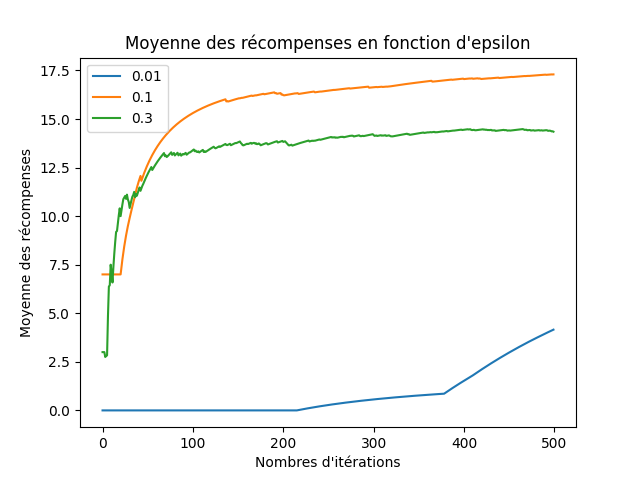
\includegraphics[width=0.7\textwidth,height=\textheight]{./img/etat_de_lart/decision_markov/moy_exploration_exploitation.png}
\caption{Graphique de moyennes des récompenses perçues en fonction d'une
probabilité Epsilon}
\end{figure}

Pour une probabilité \(\epsilon = 0.01\), mon chercheur n'explore pas
assez et ne connaît donc pas assez rapidement dans le temps quels sont
les filons les plus rentables.

Pour une probabilité \(\epsilon = 0.3\), mon chercheur trouve très
rapidement les bons filons. Mais à long terme, la moyenne des
récompenses ne croît plus puisqu'il explore trop souvent et n'exploite
pas assez.

Lorsque mon chercheur explore avec une probabilité \(\epsilon = 0.1\),
on remarque qu'à long terme, elle représente la probabilité la plus
optimale parmi les trois.

\hypertarget{estimations-des-actions}{%
\subsubsection{Estimations des actions}\label{estimations-des-actions}}

Reprenons l'exemple précédent et imaginons que mon chercheur fait une
estimation de la valeur de l'or sur chacun des filons.

Toujours selon une probabilité \(\epsilon\), si le chercheur décide
d'explorer, il améliore l'estimation du filon sur lequel il explore.
L'estimation converge vers la vraie valeur du filon.

Plus ce filon d'or sera choisis lors de l'exploration, plus l'estimation
convergera vers la vraie valeur.

Ci-dessous le graphique, donné par le programme
\ref{exploration_exploitation_estimations}, affiche les moyennes des
récompenses obtenues par le chercheur avec les probabilités
\(\epsilon = 0\) et \(\epsilon = 0.1\) :

\begin{figure}
\centering
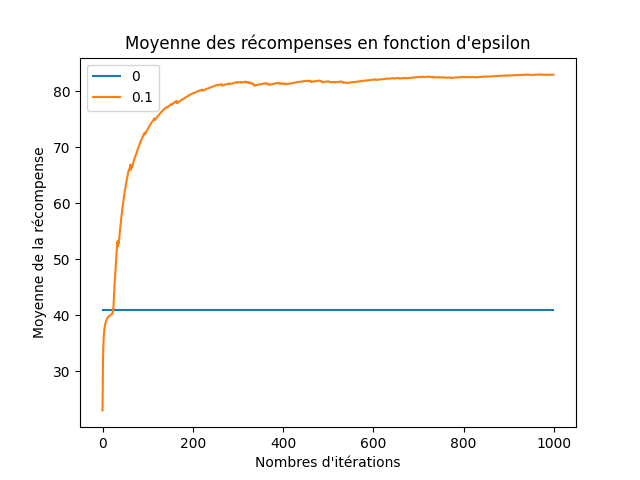
\includegraphics[width=0.7\textwidth,height=\textheight]{./img/etat_de_lart/decision_markov/moy_methode_estimation_action.png}
\caption{Graphique de moyennes des récompenses perçues en fonction
d'Epsilon avec la méthode d'estimation d'action}
\end{figure}

Lorsque la probabilité est de \(0\), le chercheur n'explore jamais, il
ne fait qu'exploiter le filon dont l'estimation qu'il a réalisée est la
plus élevée. Il n'améliore jamais ses estimations.

On appelle ce genre d'action : les actions gloutonnes.

Si la probabilité est \(\epsilon = 0.1\), le chercheur améliore au fur
et à mesure ses estimations et pourrait, à long terme, découvrir un
filon dont l'estimation était éronnée et dont la récompense réelle est
plus élevée et ainsi choisir l'action la plus optimale.

\hypertarget{suxe9lection-daction-uxe0-limite-de-confiance-supuxe9rieure}{%
\subsubsection{Sélection d'action à limite de confiance
supérieure}\label{suxe9lection-daction-uxe0-limite-de-confiance-supuxe9rieure}}

Dès lors que des estimations ont été créées, il est encore possible
d'améliorer le choix de l'action.

Si à un instant \(t\), l'action la plus optimale est \(a\) et \(a'\) une
autre action dont la valeur est proche de celle de \(a\) et dont
l'incertitude est grande. C'est-à-dire, lorsque l'action \(a'\) a été
très peu souvent choisie et donc lorsque la valeur de l'estimation de
l'action \(a'\) n'a pas été améliorée.

Alors, il est préférable de choisir \(a'\) plutôt que \(a\) car elle a
le potentiel d'être l'action la plus optimale si son estimation est
améliorée.

\hypertarget{algorithme-de-colonies-de-fourmis}{%
\subsection{Algorithme de colonies de
fourmis}\label{algorithme-de-colonies-de-fourmis}}

\hypertarget{origine-de-lalgorithme}{%
\subsubsection{Origine de l'algorithme}\label{origine-de-lalgorithme}}

Il a été proposé pour la première fois dans les années 1990 dans
l'article de recherche (A. Colorni 1990).

L'algorithme de colonies de fourmis est un algorithme permettant de
résoudre le problème de recherche de chemin de poids minimal dans un
graphe.

L'idée provient de l'observation du comportement des fourmis
lorsqu'elles cherchent un chemin entre leur colonie et une source de
nourriture.

Les biologistes ont également observé que lorsque plusieurs chemins
existaient entre la colonie et la source de nourriture, à terme, les
fourmis finissaient toujours par prendre le chemin le plus court.

Voici le comportement observé des fourmis :

\begin{enumerate}
\def\labelenumi{\arabic{enumi}.}
\item
  Une fourmi parcourt au hasard son environnement.
\item
  Si elle découvre une source de nourriture, elle revient alors à la
  colonie en déposant des phéromones d'attirance sur son chemin.
\end{enumerate}

Les fourmis se servent de phéromones pour communiquer entre elles, en
l'occurence, une phéromone d'attirance permet d'attirer d'autres
fourmis.

\begin{enumerate}
\def\labelenumi{\arabic{enumi}.}
\setcounter{enumi}{2}
\item
  Les fourmis passant à proximité auront tendance à suivre la piste.
\item
  Après avoir trouvé la nourriture et en revenant au nid, ces mêmes
  fourmis vont renforcer la piste en déposant à leurs tours des
  phéromones.
\end{enumerate}

Par définition, si une fourmi emprunte le chemin le plus court, elle
fera plus vite son aller-retour que les fourmis ayant emprunté un chemin
plus long.

Le chemin court sera donc de plus en plus renforcé, et donc de plus en
plus attractif.

Le chemin long sera oublié et finira par disparaître, les phéromones
s'étant évaporées avec le temps.

\hypertarget{lalgorithme-colonies-de-fourmis-est-un-algorithme-dapprentissage-par-renforcement}{%
\subsubsection{L'algorithme colonies de fourmis est un algorithme
d'apprentissage par
renforcement}\label{lalgorithme-colonies-de-fourmis-est-un-algorithme-dapprentissage-par-renforcement}}

L'ensemble des fourmis de la colonie sont les agents IA, la zone
naturelle entre le nid et la nourriture est l'environnement dans lequel
les agents évoluent.

Lorsqu'une fourmi décide de prendre un certain chemin jusqu'à la
nourriture, elle réalise une action. L'ensemble des actions possible est
l'ensemble des chemins empruntables par les fourmis.

Parmi l'ensemble des chemins possibles, si une fourmi emprunte un chemin
déjà utilisé, elle exploite ce chemin. Si elle emprunte un chemin encore
jamais utilisé, on dit alors qu'elle explore.

On récompense le chemin emprunté en lui attribuant des phéromones.

On dit alors qu'on renforce le chemin utilisé.

\hypertarget{modelisation-de-lalgorithme-de-colonies-de-fourmis}{%
\subsubsection{Modelisation de l'algorithme de colonies de
fourmis}\label{modelisation-de-lalgorithme-de-colonies-de-fourmis}}

Le programme \ref{colonies_fourmis} modélise l'algorithme de colonies de
fourmis.

\hypertarget{environnement}{%
\paragraph{Environnement}\label{environnement}}

L'environnement dans lequel l'algorithme de colonies de fourmis
s'effectue peut être modélisé par un graphe représentant les différents
chemins possibles menant de la colonie à la source de nourriture.

\begin{figure}
\centering
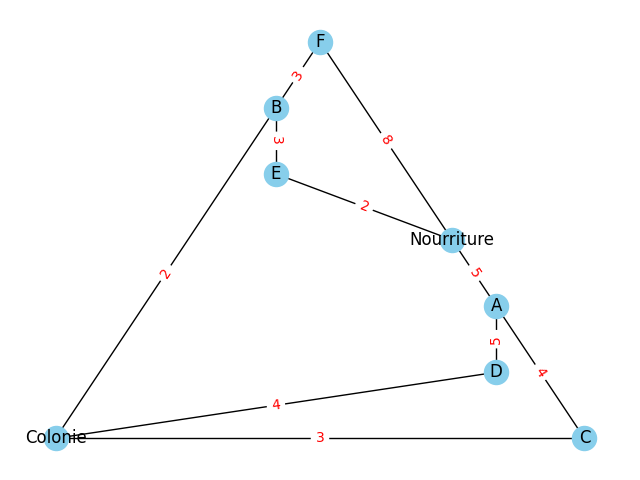
\includegraphics[width=0.7\textwidth,height=\textheight]{./img/etat_de_lart/colonies_fourmis/visualisation_graph.png}
\caption{Représentation sagitalle du graphe G}
\end{figure}

Le graphe \(G\) est un exemple de représentation sagitalle du graphe sur
lequel on va travailler tout au long de ce chapitre.

C'est un graphe connexe non orienté pondéré contenant deux poids : celui
qui est présenté sur la figure plus haut illustre le nombre de cases
qu'il faut parcourir d'un sommet \(u\) à un sommet \(v\). Le second
poids décrit le nombre de phéromones déposées sur l'arête \((u,v)\) et
sont tous initialisés à \(1\) au début de l'entrainement.

Le graphe \(G\) est représenté en machine par une liste d'adjacence :

\begin{lstlisting}[language=Python, numbers=left, caption={Liste d adjacence}]
Colonie :
   {'arrivee': 'B', 'nombre de case': 2, 'pheromones': 1}
   {'arrivee': 'C', 'nombre de case': 3, 'pheromones': 1}
   {'arrivee': 'D', 'nombre de case': 4, 'pheromones': 1}
B :
   {'arrivee': 'Colonie', 'nombre de case': 2, 'pheromones': 1}
   {'arrivee': 'E', 'nombre de case': 3, 'pheromones': 1}
   {'arrivee': 'F', 'nombre de case': 3, 'pheromones': 1}
C :
   {'arrivee': 'Colonie', 'nombre de case': 3, 'pheromones': 1}
   {'arrivee': 'A', 'nombre de case': 4, 'pheromones': 1}
D :
   {'arrivee': 'Colonie', 'nombre de case': 4, 'pheromones': 1}
   {'arrivee': 'A', 'nombre de case': 5, 'pheromones': 1}
E :
   {'arrivee': 'B', 'nombre de case': 3, 'pheromones': 1}
   {'arrivee': 'Nourriture', 'nombre de case': 2, 'pheromones': 1}
F :
   {'arrivee': 'B', 'nombre de case': 3, 'pheromones': 1}
   {'arrivee': 'Nourriture', 'nombre de case': 8, 'pheromones': 1}
A :
   {'arrivee': 'C', 'nombre de case': 4, 'pheromones': 1}
   {'arrivee': 'D', 'nombre de case': 5, 'pheromones': 1}
   {'arrivee': 'Nourriture', 'nombre de case': 5, 'pheromones': 1}
Nourriture :
   {'arrivee': 'A', 'nombre de case': 5, 'pheromones': 1}
   {'arrivee': 'E', 'nombre de case': 2, 'pheromones': 1}
   {'arrivee': 'F', 'nombre de case': 8, 'pheromones': 1}
\end{lstlisting}

\hypertarget{fourmis-artificielles}{%
\paragraph{Fourmis artificielles}\label{fourmis-artificielles}}

Les fourmis artificielles diffèrent des fourmis réelles. Ces différences
sont mises en avant dans la thèse (Nonmarché 2000).

Les fourmis artificielles possèdent une mémoire, ne sont pas totalement
aveugles et ne font pas autre chose que ce qu'on leur a demandé.

Dès que la fourmi artificielle trouve la nourriture, elle revient
automatiquement vers la colonie.

Une fourmi artificielle se souvient du chemin qu'elle a emprunté et
enlève les cycles, c'est pour cela qu'elle est dotée d'une mémoire.

Une fourmi dépose une trace de phéromones sur l'arête \((u,v)\) quand
elle arrive au sommet \(v\). Elle dépose ses phéromones uniquement après
avoir trouvé la nourriture.

La fourmi artificielle possède les attributs suivants :

\begin{itemize}
\item
  Un numéro d'identification
\item
  Un chemin, sans cycles, contenant les sommets qu'elle a traversé
\item
  Un entier signifiant le nombre de cases qu'il lui reste à parcourir
  pour atteindre le sommet \(v\) dans l'arête \((u,v)\)
\item
  Un booléen indiquant si elle a trouvé la nourriture
\item
  Un entier représentant le nombre total de cases à parcourir sur le
  retour
\end{itemize}

Elle possède également plusieurs méthodes lui permettant :

\begin{itemize}
\item
  D'avancer d'une case
\item
  De revenir vers la colonie d'une case
\item
  De savoir si elle est sur un sommet
\item
  De savoir si elle est sur le sommet de nourriture
\item
  De savoir si elle est sur le sommet de colonie
\end{itemize}

Une fourmi artificielle sera une instanciation de la classe
\passthrough{\lstinline!Fourmi!} :

\begin{lstlisting}[language=Python, numbers=left, caption={Classe Fourmi}]
class Fourmi:
    def __init__(self,numero : int,s_de_depart : str):
        """
        Constructeur : Initialise une fourmi a partir d'un numero de fourmi et d'un sommet de depart
        """
        self.numero = numero
        self.chemin = [s_de_depart]
        self.nb_cases = 0
        self.nb_cases_retour = 0
        self.retour = False

    def avancer(self):
        """
        Avance d'une case la fourmi
        """
        self.nb_cases -= 1

    def revenir(self):
        """
        Avance d'une case la fourmi lorsqu'elle revient a la colonie
        """
        self.nb_cases_retour -= 1

    def est_sur_sommet(self)->bool:
        """
        :return booleen: Renvoie True si la fourmi est sur un sommet, False sinon
        """
        return self.nb_cases == 0

    def est_sur_nourriture(self)->bool:
        """
        :return booleen: Renvoie True si la fourmi est sur le sommet de nourriture, False sinon
        """
        return self.chemin[-1] == 'Nourriture'

    def est_revenue(self):
        """
        :return booleen: Renvoie True si la fourmi est revenue a la colonie, False sinon
        """
        return self.nb_cases_retour == 0
\end{lstlisting}

\hypertarget{choix-du-voisin}{%
\paragraph{Choix du voisin}\label{choix-du-voisin}}

Lorsqu'une fourmi est arrivée à un sommet \(u\), elle va effectuer un
choix aléatoire pondéré sur tous les voisins \(v\) de \(u\) selon la
quantité de phéromones déposée sur l'arête \((u,v)\). La fonction
\protect\hyperlink{choix_voisin}{choix\_voisin} permet de réaliser un
tel comportement :

\begin{lstlisting}[language=Python, numbers=left, caption={Choix du voisin}]
def choix_voisin(model : dict,sommet_courant : str)->str:
    """
    :param model (dict): Graphe G represente par une liste d'adjacence
    :param sommet_courant (str): Un sommet u de G
    :return str: un sommet aleatoire voisin de u
    """
    voisins = model.voisins(sommet_courant)
    voisins_nom = [v["arrivee"] for v in voisins]
    voisins_pheromones = [v["pheromones"] for v in voisins]
    return random.choices(voisins_nom, weights=voisins_pheromones, k=len(voisins_pheromones))[0]
\end{lstlisting}

\hypertarget{renforcement-du-chemin}{%
\paragraph{Renforcement du chemin}\label{renforcement-du-chemin}}

Une fois qu'une fourmi est rentrée à la colonie, c'est-à-dire, une fois
qu'elle a atteint le sommet \(Colonie\) sur son retour. Le chemin
\(Nourriture \rightarrow Colonie\) sera renforcé de \(1\) phéromone.

C'est la fonction
\protect\hyperlink{renforcer_chemin}{renforcer\_chemin} qui effectue
cette opération :

\begin{lstlisting}[language=Python, numbers=left, caption={Renforcement du chemin}]
def renforcer_chemin(model : dict,chemin : list):
    """
    :param model (dict): Graphe G represente par une liste d'adjacence
    :param chemin (list): Liste contenant tous les sommets que la fourmi a traverse
    """
    for i in range(0,len(chemin)-1):
        iv = model.get_indice_voisin(chemin[i],chemin[i+1])
        model.adj[chemin[i]][iv]["pheromones"] += 1
\end{lstlisting}

\hypertarget{uxe9vaporation}{%
\paragraph{Évaporation}\label{uxe9vaporation}}

L'évaporation des phéromones s'effectue à une fréquence de \(x\) tours
et est très importante puisqu'elle permet de faire disparaître les
chemins plus longs qui auraient été renforcés par quelques
exploratrices. La fonction \protect\hyperlink{evaporation}{evaporation}
permet de faire enlever \(1\) phéromone sur toutes les arêtes du graphe
:

\begin{lstlisting}[language=Python, numbers=left, caption={Frequence d evaporation}]
def evaporation(model : dict):
    """
    :param model (dict): Graphe G represente par une liste d'adjacence
    """
    for k in model.adj :
        for i in range(len(model.adj[k])):
            if model.adj[k][i]["pheromones"] > 1:
                model.adj[k][i]["pheromones"] -= 1
\end{lstlisting}

\hypertarget{algorithme-principal}{%
\paragraph{Algorithme principal}\label{algorithme-principal}}

L'algorithme des colonies de fourmis est un algorithme d'apprentissage
par renforcement, il fonctionne alors dans le temps. Chaque pas de temps
\(t\) correspond à un tour de jeu, \(n\) étant le nombre total de tours
de jeu que l'on s'est fixé.

\begin{lstlisting}[numbers=left, caption={Algorithme Colonies de fourmis}]
Procedure colonie_de_fourmis
Entrees : un graphe G

liste_fourmis <- ensemble vide
Pour i allant de 0 a n faire :
    Ajouter Fourmi() a liste_fourmis
    Pour chaques fourmis f de liste_fourmis faire :
        Si f est sur le retour et si f est arrivee a la colonie alors :
            Renforcer le chemin de f
            Enlever f de liste_fourmis
        Sinon si f est arrivee a un sommet s alors :
            Si s est la source de nourriture alors :
                f est sur le retour
                Nombre de cases a parcourir pour f <- Somme w(u,v) avec (u,v) l'ensemble des aretes du chemin de f
            Sinon :
                sommet_suivant <- choix_voisin(G,s)
                Nombre de cases a parcourir pour f <- w(s,sommet_suivant)
                Ajouter sommet_suivant a chemin de f
        Avancer d'une case la fourmi f
    Si i est un tour d'evaporation alors:
        evaporation(G)
\end{lstlisting}

\hypertarget{optimisation-des-paramuxe8tres}{%
\paragraph{Optimisation des
paramètres}\label{optimisation-des-paramuxe8tres}}

Les statistiques suivantes ont été réalisées à partir du graphe \(G\).

Plusieurs paramètres dans l'algorithme permettent de varier le
pourcentage de réussite comme le nombre de fourmis utilisées et la
fréquence d'utilisation de l'évaporation.

Une partie est considérée comme gagnée, si les phéromones sont plus
nombreuses sur le chemin le plus court.

\begin{figure}
\centering
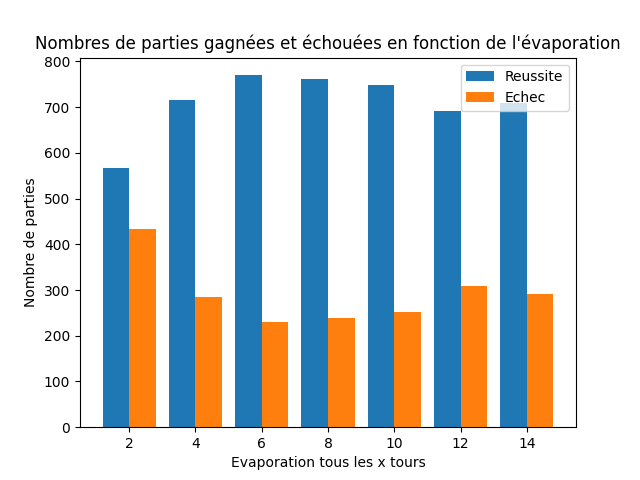
\includegraphics[width=0.7\textwidth,height=\textheight]{./img/etat_de_lart/colonies_fourmis/optimisation_parametres/nb_parties_evaporation.png}
\caption{Graphique sur l'optimisation de fréquence d'évaporation}
\end{figure}

Sur ce graphique sont représentés le nombre de parties gagnée et
échouées en fonction de la fréquence d'évaporation. On remarque sur ce
graphique que le pourcentage de réussite est optimal lorsque
l'évaporation s'effectue tous les 6-8 tours.

\begin{figure}
\centering
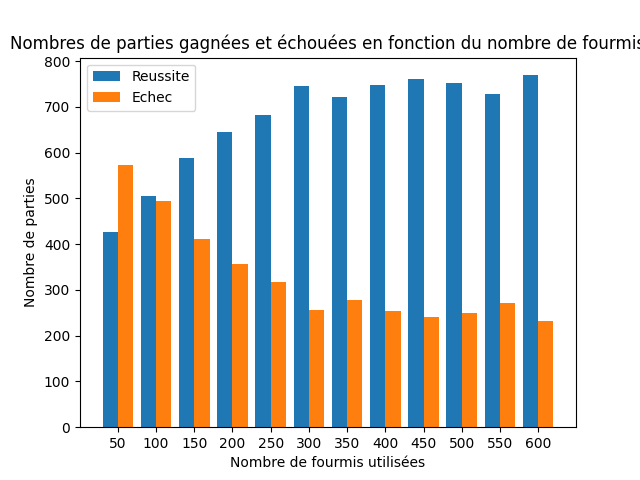
\includegraphics[width=0.7\textwidth,height=\textheight]{./img/etat_de_lart/colonies_fourmis/optimisation_parametres/nb_parties_fourmis.png}
\caption{Graphique sur l'optimisation du nombre de fourmis déployées}
\end{figure}

Sur ce graphique sont représentés le nombre de parties gagnées et
échouées en fonction du nombre de fourmis employées. On remarque sur ce
graphique que le pourcentage de réussite est optimal à partir de 300
fourmis utilisées.

\hypertarget{statistiques-de-ruxe9ussite}{%
\paragraph{Statistiques de réussite}\label{statistiques-de-ruxe9ussite}}

Les statistiques suivantes ont été réalisées à partir du graphe \(G\)
avec \(n\) le nombre de fourmis \(n = 500\) et avec \(e\) le nombre de
tours séparant chaques évaporations \(e = 8\).

\begin{figure}
\centering
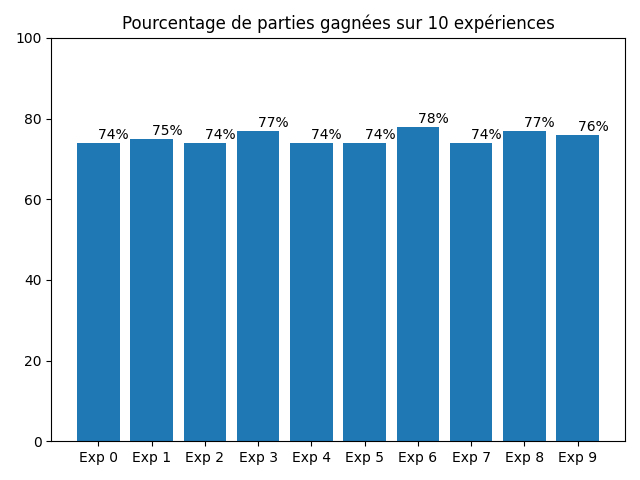
\includegraphics[width=0.7\textwidth,height=\textheight]{./img/etat_de_lart/colonies_fourmis/statistiques/pourcentage_reussite.png}
\caption{Graphique représentant le pourcentage de réussite de 10
expériences}
\end{figure}

Sur le graphique de la figure ci-dessus sont représentés les
pourcentages de réussite de 10 expériences. Chaques expériences calcule
le pourcentage de réussite de 500 parties.

On remarque que la réussite varie entre 70\% et 80\%.

\begin{figure}
\centering
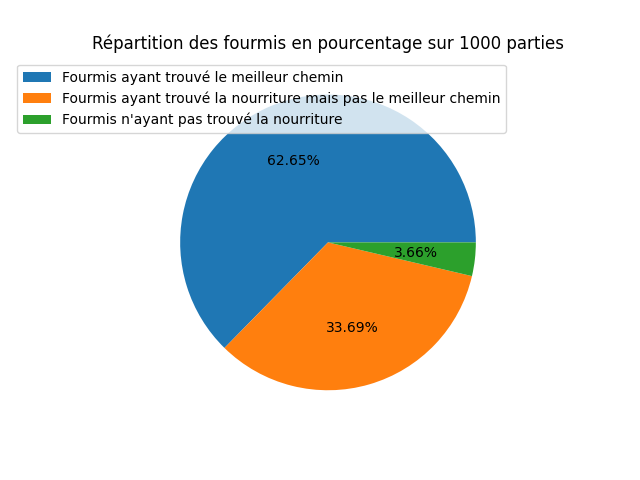
\includegraphics[width=0.7\textwidth,height=\textheight]{./img/etat_de_lart/colonies_fourmis/statistiques/repartition_fourmis.png}
\caption{Graphique de répartition en moyenne des fourmis sur 1000
parties}
\end{figure}

Sur la précédente figure sont représentés l'état en pourcentage de
chaques fourmis pour 1000 parties.

Les 4\% de fourmis qui n'ont pas trouvé la nourriture sont celles encore
présentes dans le graphe après l'issue de la partie. Ce sont celles qui
ont été ajoutées peu avant la fin de la partie.

Les fourmis ayant trouvé la nourriture mais en n'ayant pas emprunté le
meilleur chemin sont à 33\% du total des fourmis, ce qui peut paraître
beaucoup lorsque que sur 1000 parties, il y a environ 75\% de réussite.

Cela s'explique par le fait que les fourmis explorent beaucoup en début
de partie et trouvent un chemin long.

Avec l'évaporation, les chemins longs disparaissent dans le temps et
font qu'une partie réussisse quand même.

Mais le fait est que ces chemins sont quand même comptabilisés dans le
pourcentage de fourmis n'ayant pas trouvé le chemin le plus court.

\begin{figure}
\centering
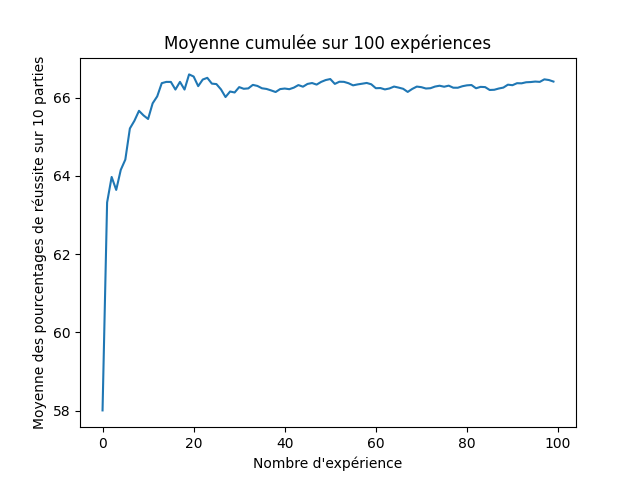
\includegraphics[width=0.7\textwidth,height=\textheight]{./img/etat_de_lart/colonies_fourmis/statistiques/moy_cumul.png}
\caption{Moyenne cumulée de 100 expériences}
\end{figure}

Sur la figure ci-dessus est représenté la moyenne cumulée de 100
expériences.

Chaque expérience se réalise sur 100 parties : on calcule la moyenne du
pourcentage de réussite sur ces 10 parties, c'est-à-dire le pourcentage
de fourmis ayant trouvé le meilleur chemin.

Le tracé de courbe de la figure 7 semble converger vers 66, ce qui
laisse penser que l'algorithme reste fiable dans le temps.

\hypertarget{reconnaissance-de-caractuxe8res-manuscrits}{%
\subsection{Reconnaissance de caractères
manuscrits}\label{reconnaissance-de-caractuxe8res-manuscrits}}

La reconnaissance de caractères manuscrits est souvent utilisée dans les
banques afin de vérifier l'authenticité des chèques notamment.

Plus tard, la reconnaissance de caractères manuscrits pourrait être
utilisée pour retrouver l'identité d'une personne à partir de son
écriture.

\hypertarget{pruxe9sentation-du-probluxe8me}{%
\subsubsection{Présentation du
problème}\label{pruxe9sentation-du-probluxe8me}}

La reconnaissance de caractères manucrits (ou \emph{Handwritten
Characters Recognition}) est un problème dérivant du problème de
reconnaissance de formes.

C'est l'ensemble des techniques visant à identifier des régularités à
partir de données brutes afin de prendre une décision pour classifier le
motif.

Il s'agit donc d'un problème de classification.

Soit \emph{F} l'image d'un caractère quelconque \emph{c}, la
reconnaissance de caractères manuscrits (HCR) est capable de reconnaître
et classifier ainsi le caractère : \(HCR(F) = c\)

Il existe plusieurs problèmes de reconnaissance de caractères dont la
reconnaisance en ligne et hors ligne.

Lors de la reconnaissance en ligne, l'utilisateur est directement
connecté à un crayon électronique et la reconnaissance s'effectue en
direct. L'odrinateur observe le sens d'écriture et est alors capable de
reconnaître le caractère en utilisant des vecteurs le long du tracé.

En reconnaissance hors ligne, elle s'effectue à partir d'une photo du
caractère. On ne connaît donc pas le sens d'écriture. La méthode pour
reconnaître un caractère décrite dans ce chapitre ne concerne donc que
le problème de reconnaissance hors-ligne.

Une résolution au problème de reconnaissance hors ligne a été étudié
dans l'article (Pant 2012) et utilise les réseaux de neuronnes (ou
Neural Networks) ou plus précisément un Perceptron.

\hypertarget{pruxe9-traitement-de-limage}{%
\subsubsection{Pré-traitement de
l'image}\label{pruxe9-traitement-de-limage}}

La donnée, l'image du caractère, doit être exploitable pour pouvoir
utiliser la méthode de reconnaissance hors-ligne et les réseaux de
neurones.

Pour rendre l'image exploitable, il convient d'effectuer plusieurs
pré-traitements.

Le premier consiste à corriger les défauts ``naturels'' de l'image, il
faut entre autre corriger l'inclinaison de l'image de sorte que le
caractère soit horizontal ou la netteté des tracés.

Le second pré-traitement rends l'image exploitable en machine.

Ci-dessous un algorithme de pré-traitement de l'image.

```\{\\
Procedure pre\_traitement\_image\\
Entrees : une image d'un caractere

Lire l'image\\
Convertir l'image RGB en image en noir et blanc\\
Suppression (mettre en blanc) des pixels inutiles a l'aide d'un
filtrage\\
Convertir en image binaire\\
Inversion du noir et du blanc\\
Suppression des pixels autour du caractere\\
Normalisation des dimensions de l'image (36x36 par exemple)\\
Squelettisation des traces (un pixel en largeur du trace)

\begin{lstlisting}

![Image debut RGB a Image fin pre traitement](./img/etat_de_lart/perceptron/pre_traitement/pre_traitement_image.PNG){width=70%}

### Réseaux de neurones

L'idée du réseau de neurones émerge pour la première fois dans les années 1940 par les neurologues W. McCulloch et W. Pitts puis est repris et amélioré par D. Hebb dans son ouvrage [@TheOrganizationofBehevior].

À la suite de cet article, F. Rosenblatt invente le modèle du Perceptron en 1958. C'est le premier système artificiel de réseau de neurones à une couche capable d'apprendre par expérience.

Le Perceptron est fortement inspiré du fonctionnement des neurones biologiques.

#### Neurones biologiques

Le système nerveux est composé de milliards de cellules : c'est un réseau de neurones biologiques où chaque neurone transmet de l'information à d'autres neurones via impulsion électrique.

L'information est d'abord reçue par des capteurs appelés dendrites dans le corps cellulaire.

Puis elle est acheminée par l'axone pour atteindre les synapses à l'extrémité de la terminaison neuronale afin d'être reconduite à un autre neurone.

![Neurone biologique](./img/etat_de_lart/perceptron/reseau_de_neurones/neurone_biologique.png){width=70%}

Les neurones biologiques disposent d'un centre de contrôle faisant la somme des informations recueillies par les dendrites.

- Si la somme ne dépasse pas le seuil d'excitation : pas de message nerveux.

- Si la somme dépasse le seuil d'excitation : un message nerveux est émis via l'axone au neurone suivant.

#### Réseau de Neurones artificiels

Un réseau de neurones artificiels est un ensemble de neurones connectés entre eux. On distingue trois familles de couche de neurones :

- La famille des entrées (ou *Inputs*) coloriés en vert sur la figure.

- La famille des couches cachées (ou *Hidden Layers*) coloriés en bleu.

- Puis la famille des sorties (ou *Outpouts*) coloriés en jaune.

![Réseau de neurones artificiels](./img/etat_de_lart/perceptron/reseau_de_neurones/reseau_de_neurones_artificiels.png){width=50%}

Les neurones (sauf ceux des entrées) sont liés avec tous les neurones de la couche précédente. Il n'y a qu'une couche cachée pour le Perceptron, mais il existe des réseaux plus performants à plusieurs couches cachées.

#### Principe de Feed Forward

Dans les réseaux de neurones artificiels, on attribut aux entrées des données. Les données sont transmises d'une couche à une autre en respectant le principe du Feed Forward.

Ci-dessous, le schéma d'un neurone artificiel $j$ :

![Principe de Feed Forward du neurone artificiel j](./img/etat_de_lart/perceptron/reseau_de_neurones/neurone_artificiel_feed_forward.png){width=80%}

Soit $(X_1,X_2, ..., X_n)$, les valeurs attribuées aux précédents neurones de $j$.

Et $(W_{1j}, W_{2j}, ..., W_{nj})$ les poids respectifs des vecteurs de poids des neurones prédécésseurs de $j$.

Soit $net_j$ la valeur calculée par la fonction de combinaison du neurone $j$ :

$net_j =\sum_{i=1}^{n}X_i \times W_i$

Le neurone calcule la valeur $net_j$, il va ensuite pouvoir la modifier selon une fonction d'activation  $\varphi$

La fonction d'activation est une fonction qui va déterminer si le neurone s'active ou non.

Si la valeur calculée par la fonction d'activation : $\varphi(net_j)$ n'est pas supérieure au seuil $\theta_j$, le neurone ne s'active pas et la valeur ne passe pas aux prochains neurones.

Si, au contraire, la valeur calculée par la fonction d'activation est supérieure au seul $\theta_j$, le neurone s'active et la valeur passe aux prochains neurones.

Le neurone a également la possibilité d'ajouter à l'entrée de la fonction d'activation un biais. Cela permet au neurone d'avoir de l'influence sur la fonction d'activation.

#### Fonction d'erreur

Au début, les valeurs renvoyées par les neurones de sortie ne sont pas celles auquelles on attendait, c'est normal puisque le réseau n'est pas entraîné.

C'est ici qu'intervient le principe d'apprentissage par renforcement : grâce à une fonction d'erreur, le réseau va pouvoir mettre à jour, renforcer les poids des vecteurs de telle façon à ce que les valeurs renvoyées par les neurones de sortie deviennent vraies.

La fonction d'erreur permet de savoir à quel point la valeur de sortie est différente de celle attendue.

Soit $t$ la valeur attendue et $out$ la valeur de sortie, la fonction d'erreur $e$ s'écrit : $e = \frac{1}{2}(t-out)^2$

Ainsi, plus la différence est importante entre $t$ et $out$, plus $e$ est grand.

Lorsqu'il n'y a pas d'erreur, $e$ est proche de $0$. Dans le cas contraire, il faut donc modifier les vecteurs de poids de sorte que $e$ se rapproche de $0$.

Pour cela, le réseau va utiliser ce qu'on appelle la rétro-propagation.

L'idée est d'identifier les vecteurs qui ont une énorme influence sur la valeur de sortie et de les réduire proportionnellement à l'impact qu'ils ont sur $e$.

### Méthode de reconnaissance de caractères utilisant un Perceptron

L'idée est d'utiliser un réseau de neurones simple, le Perceptron, où chaque entrée est définie par un pixel de l'image. On dit, par exemple, que la valeur de l'entrée est 0 si le pixel est noir et 100 si le pixel est blanc.

Puis, en sortie, les valeurs des probabilités de la classification de l'image.

![Reconnaissance de caractère manuscrit utilisant un Perceptron](./img/etat_de_lart/perceptron/perceptron_reconnaissance_caractere_manuscrit/perceptron_reconnaissance_caractere_manuscrit.PNG){width=100%}

### Méthode de reconnaissance de caractères utilisant un CNN

En utilisant un Perceptron, il y a autant d'entrées que de pixels dans l'image. Donc pour une image aux dimensions classiques telles que 1366x768 necessiterait plus d'un million d'entrées.

Le Réseau de Neurones Convolutionnels (ou *Convolutional Neural Network*) est une sous-catégorie de réseau de neurones répondant plus efficacement au problème. Il réponds même de manière générale à la reconnaissance d'image.

En plus d'un réseau de neurones utilisé comme classifieur, l'architecture d'un CNN dispose en amont d'une partie convolutive.

L'objectif final de la partie convolutive est de déterminer un code CNN de l'image.

Pour cela, il s'agit de découper en plusieurs sous-parties l'image initiale, les sous-parties ainsi crées sont alors appelées cartes de convolutions :

![Cartes de convolutions obtenues à partir de l'image initiale](./img/etat_de_lart/perceptron/CNN_reconnaissance_image/cartes_convolutions.PNG){width=40%}

Plusieurs caractéristiques de chaque carte de convolution est calculée, puis est soumise à un filtre (appelé *Max-Pooling*) afin de réduire le nombre de caractéristiques. Le filtre, présenté ci-dessous, consiste simplement à garder uniquement la plus forte caractéristique dans chaque carte de convolution :

![Effet du filtre de Max-Pooling sur chaque cartes de convolutions](./img/etat_de_lart/perceptron/CNN_reconnaissance_image/max_pooling.PNG){width=70%}

Le code CNN est alors obtenu en concaténant les caractéristiques après filtrage.

C'est ce même code CNN qui sera passé en entrée au réseau de neurones. C'est l'étape de classification de l'image.

### Implémentation avec Torch

Le module ``Torchvision`` est un module python nous permettant d'utiliser des réseaux de neurones pré-entraînés (il ne s'agit donc plus d'algorithme d'apprentissage par renforcement).

Importation des bibliothèques :

```{.python .numberLines caption="Importation des modules"}
from keras.preprocessing.image import load_img
from keras.preprocessing.image import img_to_array
from keras.applications.vgg16 import preprocess_input
from keras.applications.vgg16 import decode_predictions
from keras.applications.vgg16 import VGG16
\end{lstlisting}

Entrainement du modèle pré-entrainé VGG16 :

\begin{lstlisting}[language=Python, numbers=left, caption={Entrainement du modele}]
model = VGG16()
\end{lstlisting}

Importation de l'image à prédire :

\begin{lstlisting}[language=Python, numbers=left, caption={Importation de l image}]
img = load_img('caractere.jpg', target_size=(224, 224))
\end{lstlisting}

Pré-traitement de l'image :

\begin{lstlisting}[language=Python, numbers=left, caption={Pre traitement}]
def preprocess(image) :
    image = img_to_array(image)
    image = image.reshape((1, image.shape[0], image.shape[1], image.shape[2]))
    image = preprocess_input(image)
    return image
\end{lstlisting}

Prédiction du modèle :

\begin{lstlisting}[language=Python, numbers=left, caption={Prediction du modele}]
def pred_modele(image) :
    image = preprocess(image)
    y_pred = model.predict(image)
    label = decode_predictions(y_pred)
    label = label[0][0]
    return ((label[1], label[2]*100))

print("Prediction image:",pred_modele(img)[0], 'avec une probabilite de',pred_modele(img)[1])
\end{lstlisting}

\hypertarget{stratuxe9gie-et-muxe9thodologie-dexpuxe9rimentation}{%
\section{Stratégie et méthodologie
d'expérimentation}\label{stratuxe9gie-et-muxe9thodologie-dexpuxe9rimentation}}

Dans ce chapitre y seront détaillées la stratégie ainsi que la
méthodologie d'expérimentation afin de répondre du mieux possible à la
problèmatique posée.

Une stratégie pédagogique représente l'ensemble des méthodes
pédagogiques choisies visant à atteindre un objectif comme :

\begin{itemize}
\item
  Motiver les apprennants et les aider à se concentrer.
\item
  Organiser les informations pour que les apprennants puissent mieux les
  comprendre et les mémoriser.
\item
  Contrôler et évaluer l'apprentissage.
\end{itemize}

\emph{Problématique : Comment démystifier la vision qu'ont les élèves de
l'intelligence artificielle ?}

\hypertarget{enjeux-de-la-probluxe8matique}{%
\subsection{Enjeux de la
problèmatique}\label{enjeux-de-la-probluxe8matique}}

Ci-dessous, une liste non exhaustive d'exemple de reportages diffusés
sur de grandes chaînes de télévision françaises :

\begin{itemize}
\item
  \href{https://www.tf1info.fr/high-tech/video-reportage-tf1-etats-unis-penurie-de-main-d-oeuvre-dans-les-restaurants-mon-serveur-est-un-robot-2245198.html}{``TF1
  - Etats-Unis : mon serveur est un robot''}
\item
  \href{https://www.tf1info.fr/sciences-et-innovation/interview-chatgpt-intelligence-artificielle-qui-repousse-les-limites-du-possible-bluffant-pour-ne-pas-dire-traumatisant-en-tant-qu-humain-selon-jean-gabriel-ganascia-2244812.html}{``TF1
  - ChatGPT, l'intelligence artificielle qui repousse les limites du
  possible : « Bluffant, même traumatisant en tant qu'humain »}
\item
  \href{\%5BCash\%20Investigation\%20-\%20Au\%20secours,\%20mon\%20patron\%20est\%20un\%20algorithme\%20en\%20streaming\%20-\%20Replay\%20France\%202\%20\%7C\%20France\%20tv\%5D(https://www.france.tv/france-2/cash-investigation/1066737-au-secours-mon-patron-est-un-algorithme.html)}{``FranceTV
  - Au secours, mon patron est un algorithme''}
\item
  \href{\%5BIntelligence\%20artificielle\%20:\%20jusqu\textquotesingle{}où\%20iront\%20les\%20robots\%20humanoïdes\%20?\%20\%7C\%20TV5MONDE\%20-\%20Informations\%5D(https://information.tv5monde.com/video/intelligence-artificielle-jusqu-ou-iront-les-robots-humanoides)}{``TV5Monde
  - Intelligence artificielle : jusqu'où iront les robots humanoïdes
  ?''}
\item
  \href{\%5BIntelligence\%20artificielle\%20:\%20la\%20médecine\%20en\%20pleine\%20révolution\%20-\%20J.-E.\%20Bibault\%20-\%20Extrait\%20C\%20l\textquotesingle{}hebdo\%20en\%20streaming\%20\%7C\%20France\%20tv\%5D(https://www.france.tv/france-5/c-l-hebdo/c-l-hebdo-saison-7/4523950-intelligence-artificielle-la-medecine-en-pleine-revolution-j-e-bibault-c-l-hebdo-14-01-2023.html)}{``FranceTV
  - Intelligence artificielle : la medecine en pleine révolution''}
\end{itemize}

Ces reportages ont un thème commun : l'intelligence artificielle.

Nombre de médias écrivent des articles ou réalisent des reportages sur
l'apparition de nouvelles technologies utilisant l'intelligence
artificielle comme les voitures autonomes Tesla, il y a quelques années,
et plus récemment sur l'outil ChatGPT.

Ces reportages sont pour la plupart du temps de l'information
vulgarisée, il n'y a pas ou peu d'explications sur le fonctionnement des
algorithmes. Il y est surtout présenté les spécificités de la
technologie.

De plus, au travers du titre de l'article ou de la voix hors champs, les
médias arrivent à susciter chez les téléspectateurs une part de mystère,
de crainte voire de peur pour l'intelligence artificielle.

Les téléspectateurs, dont les élèves, construisent alors peu à peu une
vision souvent éronnée de l'intelligence artificielle. Par exemple, ils
entendent ou utilisent les termes ``machine learning'' ou
``apprentissage automatique'' sans connaître leur signification.

L'intelligence artificielle est ainsi mystifiée. Alors qu'elle est
actuellement de plus en plus présente dans nos quotidiens, nos
entreprises, nos recherches scientifiques. L'école a pour mission
d'armer les élèves de connaissances nécessaires pour comprendre le monde
sur lequel ils évoluent.

\hypertarget{objectifs}{%
\subsection{Objectifs}\label{objectifs}}

L'objectif de la séquence est de faire découvrir l'intelligence
artificielle aux élèves.

De manière plus précise :

\begin{itemize}
\item
  Faire manipuler aux apprenants un algorithme d'apprentissage par
  renforcement dans un contexte simplifié.
\item
  Faire développer les compétences de travail en équipe, on peut noter :
  la communication, la collaboration, la responsabilité ainsi que la
  mutualisation des connaissances et compétences et d'auto-organisation.
\item
  Sensibiliser et faire se questionner l'élève sur l'intelligence
  artificielle.
\end{itemize}

\hypertarget{progression}{%
\subsection{Progression}\label{progression}}

Les algorithmes d'apprentissage par renforcement et plus généralement
l'intelligence artificielle ne sont pas au programme de SNT et NSI.

Malgré cela, en NSI, la séquence peut faire lien avec un autre chapitre
comme les graphes ou la programmation orientée objet en Terminale NSI,
l'algorithme KNN (\emph{K-nearest neighbors}) qui est un algorithme
d'apprentissage supervisé en Première NSI.

La démarche de projet occupe une place importante dans les Bulletins
Officiels des trois niveaux.

\begin{figure}
\centering

\includegraphics[width=0.7\textwidth,height=\textheight]{./img/strategie/autre/BO_demarche_de_projet.PNG}
\caption{Extrait du Bulletin Officiel}
\end{figure}

On peut alors imaginer un projet de groupe où l'on demande aux élèves de
programmer en python un algorithme d'apprentissage par renforcement.

En Seconde SNT, les enjeux de la problèmatique rencontrent parfaitement
ceux de la matière notés dans le préambule :

``L'enseignement de SNT en classe de seconde a pour objet de permettre
d'appréhender les principaux concepts des sciences numériques, mais
également de permettre aux élèves, à partir d'un objet technologique, de
comprendre le poids croissant du numérique et les enjeux qui en
découlent. {[}\ldots{]} L'enseignement de sciences numériques et
technologie aide à mieux comprendre les enjeux scientifiques et
sociétaux de la science informatique et de ses applications, à adopter
un usage réfléchi et raisonné des technologies numériques dans la vie
quotidienne et à se préparer aux mutations présentes et à venir de tous
les métiers.''

Pour la suite, nous allons considérer que la séquence est à destination
des Secondes SNT.

\hypertarget{stratuxe9gie-puxe9dagogique}{%
\subsection{Stratégie pédagogique}\label{stratuxe9gie-puxe9dagogique}}

\hypertarget{puxe9dagogie-par-le-jeu}{%
\subsubsection{Pédagogie par le jeu}\label{puxe9dagogie-par-le-jeu}}

``Un jeu est une activité de loisir, physique ou psychique, qui obéit à
des règles fixées à l'avance s'appliquant à tous les joueurs, et que
l'on pratique pour se divertir et en tirer du plaisir. Un jeu comporte
un enjeu et se termine d'une clôture symbolique marquée par la victoire
d'un joueur, d'un groupe de joueur ou parfois de tous les joueurs par
l'atteinte d'un but'' de Denis Sestier, professeur
d'histoire-géographie, acdémie de Caen, 1998.

L'idée, afin de compléter les objectifs annoncés plus haut, est de faire
manipuler, en activité, un algorithme d'apprentissage par renforcement
sous forme de jeu.

On appelle ludification (ou \emph{gamification}) le fait de rendre
ludique, avec l'utilisation de mécanismes de jeu, une situation
d'apprentissage qui ne l'était pas.

Ma stratégie repose sur l'exploitation des bienfaits du jeu pédagogique,
c'est-à-dire d'une activité ludique permettant aux élèves l'acquisition
de savoirs, savoirs-faire et savoirs-être.

Premièrement, le jeu permet le développement cognitif et social. Il fait
apprendre à coopérer, à communiquer, à développer l'autonomie, à
développer des capacités d'abstraction et à favoriser l'estime de soi.

Ensuite, le jeu permet d'accéder au savoir différamment des accès
traditionnels. On lie travail et plaisir : l'élève n'a pas l'impression
de travailler. Le jeu fait appel à sa motivation intrinsèque étant donné
que l'élève travaille désormais dans le but d'obtenir une satisfaction
personnelle, celui de gagner.

Enfin, le jeu permet l'apprentissage par l'essai-erreur qui, nous
l'avons vu avec les algorithmes d'apprentissage par renforcement, est
une méthode d'apprentissage efficace et naturelle. D'autant que l'impact
émotionnel d'une situation d'échec en jeu pédagogique est moins violent
que celui d'un apprentissage classique.

Apprendre par le jeu a toutefois un gros inconvénient : Une prise de
conscience et la structuration des apprentissages est indispensable à la
fin du jeu pour que celui-ci est efficace.

\hypertarget{duxe9rouluxe9-de-la-suxe9quence}{%
\subsubsection{Déroulé de la
séquence}\label{duxe9rouluxe9-de-la-suxe9quence}}

La séquence se découpe en 2 parties principales l'une à la suite de
l'autre :

\begin{itemize}
\item
  Cours magistral (30 minutes) :

  \begin{itemize}
  \item
    Définition de l'intelligence artificielle.
  \item
    Généralités sur l'intelligence artificielle (Histoire de l'IA,
    utilisations concrètes de l'IA).
  \item
    Définition de l'apprentissage automatique et différenciation des
    algorithmes d'apprentissage supervisés et non supervisés.
  \item
    Description des algorithmes d'apprentissage par renforcement.
  \end{itemize}
\item
  Jeu pédagogique : Manipulation d'un algorithme d'apprentissage par
  renforcement : Colonies de fourmis (1 heure et 30 minutes).

  \begin{itemize}
  \tightlist
  \item
    Présentation de l'activité.
  \item
    Activité : Travail en groupe en autonomie.
  \item
    Structuration de l'apprentissage (réinvestissement des
    connaissances, démonstration avec le programme informatique,
    hypothèses, réponses).
  \end{itemize}
\end{itemize}

Au début puis à la fin de la séquence, les élèves sont soumis à un
questionnaire.

\hypertarget{muxe9thodologie-dexpuxe9rimentation}{%
\subsection{Méthodologie
d'expérimentation}\label{muxe9thodologie-dexpuxe9rimentation}}

La méthodologie ci-dessous se penche en particulier sur le
fonctionnement de l'activité.

\hypertarget{activituxe9-colonies-de-fourmis}{%
\subsubsection{Activité : Colonies de
fourmis}\label{activituxe9-colonies-de-fourmis}}

\hypertarget{pruxe9-requis}{%
\paragraph{Pré-requis}\label{pruxe9-requis}}

Il n'y a pas de pré-requis pour pouvoir réaliser l'activité.

Une connaissance élémentaire des graphes ainsi que du problème de
recherche de poids minimal dans un graphe est utile pour appuyer
davantage l'interêt de l'algorithme des Colonies de fourmis mais n'est
pas nécessaire.

\hypertarget{nature-de-lactivituxe9}{%
\paragraph{Nature de l'activité}\label{nature-de-lactivituxe9}}

Afin de mieux aborder l'algorithme, l'activité se fait sous forme d'un
jeu de société sur lequel on déplace à la main les fourmis en suivant au
fur et à mesure les règles de la notice.

Les élèves ont alors le rôle de l'ordinateur et réalisent eux-mêmes les
instructions.

L'algorithme est ainsi ``décortiqué'' en profondeur et lui permet de
comprendre précisément son fonctionnement.

L'activité se réalise en groupe de 3 ou 4 élèves.

\hypertarget{duxe9rouluxe9-de-lactivituxe9}{%
\paragraph{Déroulé de l'activité}\label{duxe9rouluxe9-de-lactivituxe9}}

\begin{itemize}
\item
  Appropriation (15-20 minutes) :

  \begin{itemize}
  \item
    Les élèves lisent individuellement une première fois la notice.
  \item
    Puis, par groupe, ils manipulent les différents supports.
  \end{itemize}
\item
  Manipulation (30-45 minutes) :

  \begin{itemize}
  \tightlist
  \item
    Les élèves sont en groupe sur un même plateau. Ils manipulent chacun
    leurs fourmis pour exécuter les instructions plus rapidement. Les
    élèves se voient attribuer un total de 10 fourmis maximum pour
    éviter l'engorgement.
  \end{itemize}
\item
  Structuration (20-30 minutes) :

  \begin{itemize}
  \item
    Regroupement des résultats.
  \item
    Hypothèses et questionnements sur les paramètres pouvant faire
    varier le taux de réussite ou d'échec.
  \item
    Démonstration avec le programme informatique.
  \end{itemize}
\end{itemize}

\hypertarget{supports-duxe9branchuxe9s}{%
\paragraph{Supports débranchés}\label{supports-duxe9branchuxe9s}}

\hypertarget{plateau-de-jeu}{%
\subparagraph{Plateau de jeu}\label{plateau-de-jeu}}

Le principal support que les élèves utilisent est le plateau de jeu.

\begin{figure}
\centering
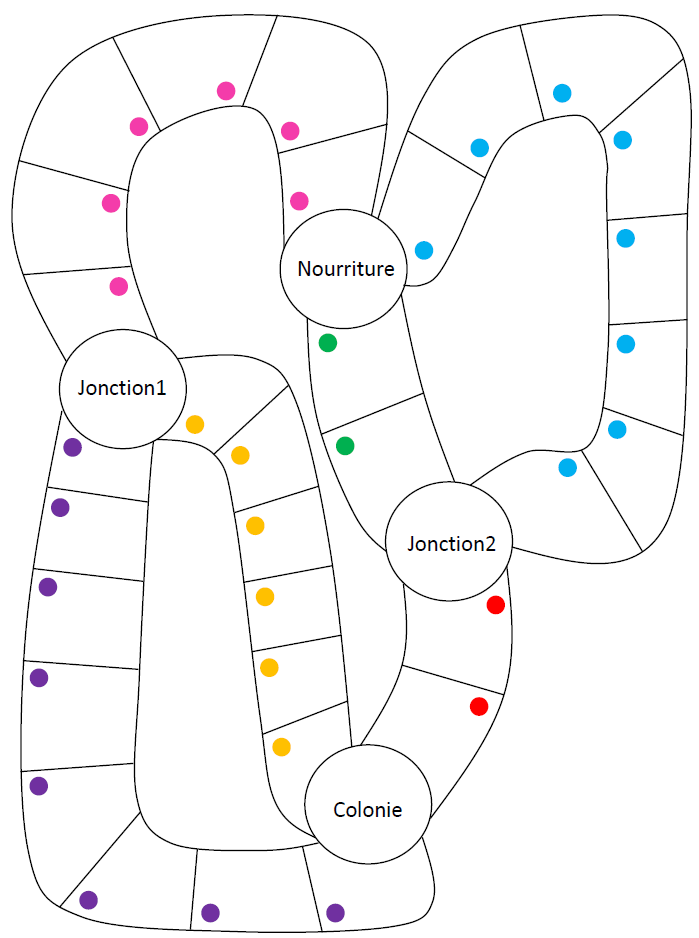
\includegraphics[width=0.8\textwidth,height=\textheight]{./img/strategie/activite/plateau.PNG}
\caption{Plateau de jeu}
\end{figure}

C'est sur ce plateau que les élèves manipulent les fourmis et tracent
les phéromones.

\hypertarget{notice-de-jeu}{%
\subparagraph{Notice de jeu}\label{notice-de-jeu}}

L'algorithme est représenté en \hyperref[sec:annexe4]{annexe 4}. sous la
forme d'une notice de jeu de société.

\hypertarget{bouxeete-des-chemins}{%
\subparagraph{Boîte des chemins}\label{bouxeete-des-chemins}}

Pour choisir représenter les sommets et leurs chemins, chaque sommet est
une boîte dans laquelle y sont placées des marqueurs. Chaques marqueurs
possèdent un symbole représentant un chemin.

Pour choisir un chemin à partir d'un sommet, l'élève tire au hasard un
marqueur de chemin depuis la boîte de ce sommet.

Lorsqu'un chemin est renforcé, on ajoute un marqueur de ce chemin dans
la boîte du sommet correspondant.

Une boîte des chemins peut être un sachet et les marqueurs des chemins,
des billes de couleurs.

\hypertarget{pions-fourmis}{%
\subparagraph{Pions fourmis}\label{pions-fourmis}}

Une fourmi est un pion sur le plateau et possède un numéro, une lettre
et une direction. Le pion est associé à un élève via la lettre.

\begin{figure}
\centering
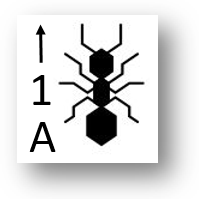
\includegraphics{./img/strategie/activite/fourmi_aller.PNG}
\caption{Fourmi n°1 de l'élève A en mode aller}
\end{figure}

Une fourmi peut être en mode ``retour'', c'est-à-dire lorsqu'elle doit
revenir à la colonie. Pour distinguer les fourmis en mode ``aller'' des
fourmis en mode ``retour'', on retourne le pion, la fourmi est d'une
autre couleur :

\begin{figure}
\centering
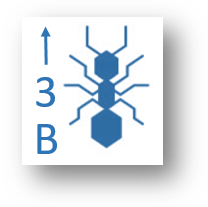
\includegraphics{./img/strategie/activite/fourmi_retour.PNG}
\caption{Fourmi n°3 de l'élève B en mode retour}
\end{figure}

\hypertarget{tableau-des-chemins}{%
\subparagraph{Tableau des chemins}\label{tableau-des-chemins}}

Une fourmi doit mémoriser les chemins par lesquels elle est passée, on
écrit alors dans le tableau des chemins, les symboles des chemins
qu'elle a emprunté :

\begin{figure}
\centering
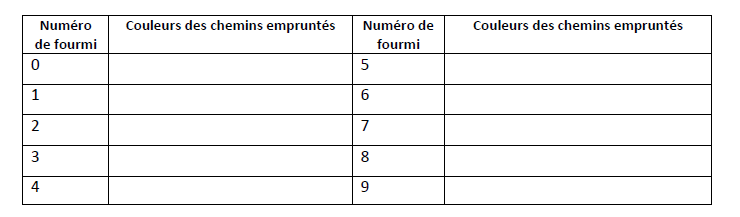
\includegraphics{./img/strategie/activite/tableau_chemins.PNG}
\caption{Tableau des chemins}
\end{figure}

\hypertarget{mise-en-commun-et-duxe9monstration}{%
\paragraph{Mise en commun et
démonstration}\label{mise-en-commun-et-duxe9monstration}}

A l'issue de la manipulation, on récupère les résultats en demandant à
chaque groupe d'élèves le chemin le plus phéromoné qu'ils ont obtenu.

Après une courte phase de débat et d'hypothèses, on affiche alors les
graphiques représentant le taux de résussite selon le nombre de fourmis
et la fréquence d'évaporation.

Puis, l'enseignant effectue une démonstration d'exécution de code
implémentant l'algorithme de colonies de fourmis.

\hypertarget{inconvuxe9nients-et-limites}{%
\paragraph{Inconvénients et limites}\label{inconvuxe9nients-et-limites}}

\begin{itemize}
\tightlist
\item
  L'execution de l'algorithme de colonies de fourmis prend beaucoup de
  temps, les algorithmes d'apprentissage par renforcement fonctionnant
  dans le temps. Il faudrait environ compter entre 50 et 60 minutes pour
  voir apparaître des résultats si l'on manipule les fourmis une par
  une.
\end{itemize}

C'est pourquoi l'activité propose de faire manipuler toutes les fourmis
de tous les élèves d'un groupe sur un tour.

\begin{itemize}
\item
  Pour ce même souci de temps, le graphe a été réfléchi de telle manière
  à ce que les fourmis atteignent ``rapidement'' la nourriture.
\item
  La notice ne correspond pas tout à fait à l'algorithme de l'état de
  l'art. En effet, dans l'activité, les fourmis ne peuvent pas choisir
  le chemin par lesquels elles viennent d'arriver.
\end{itemize}

\hypertarget{plan-de-classe}{%
\paragraph{Plan de classe}\label{plan-de-classe}}

Les groupes d'élèves sont disposés par ``ilots'' dans la salle de classe
comme le décrit la figure ci-dessous.

\begin{figure}
\centering
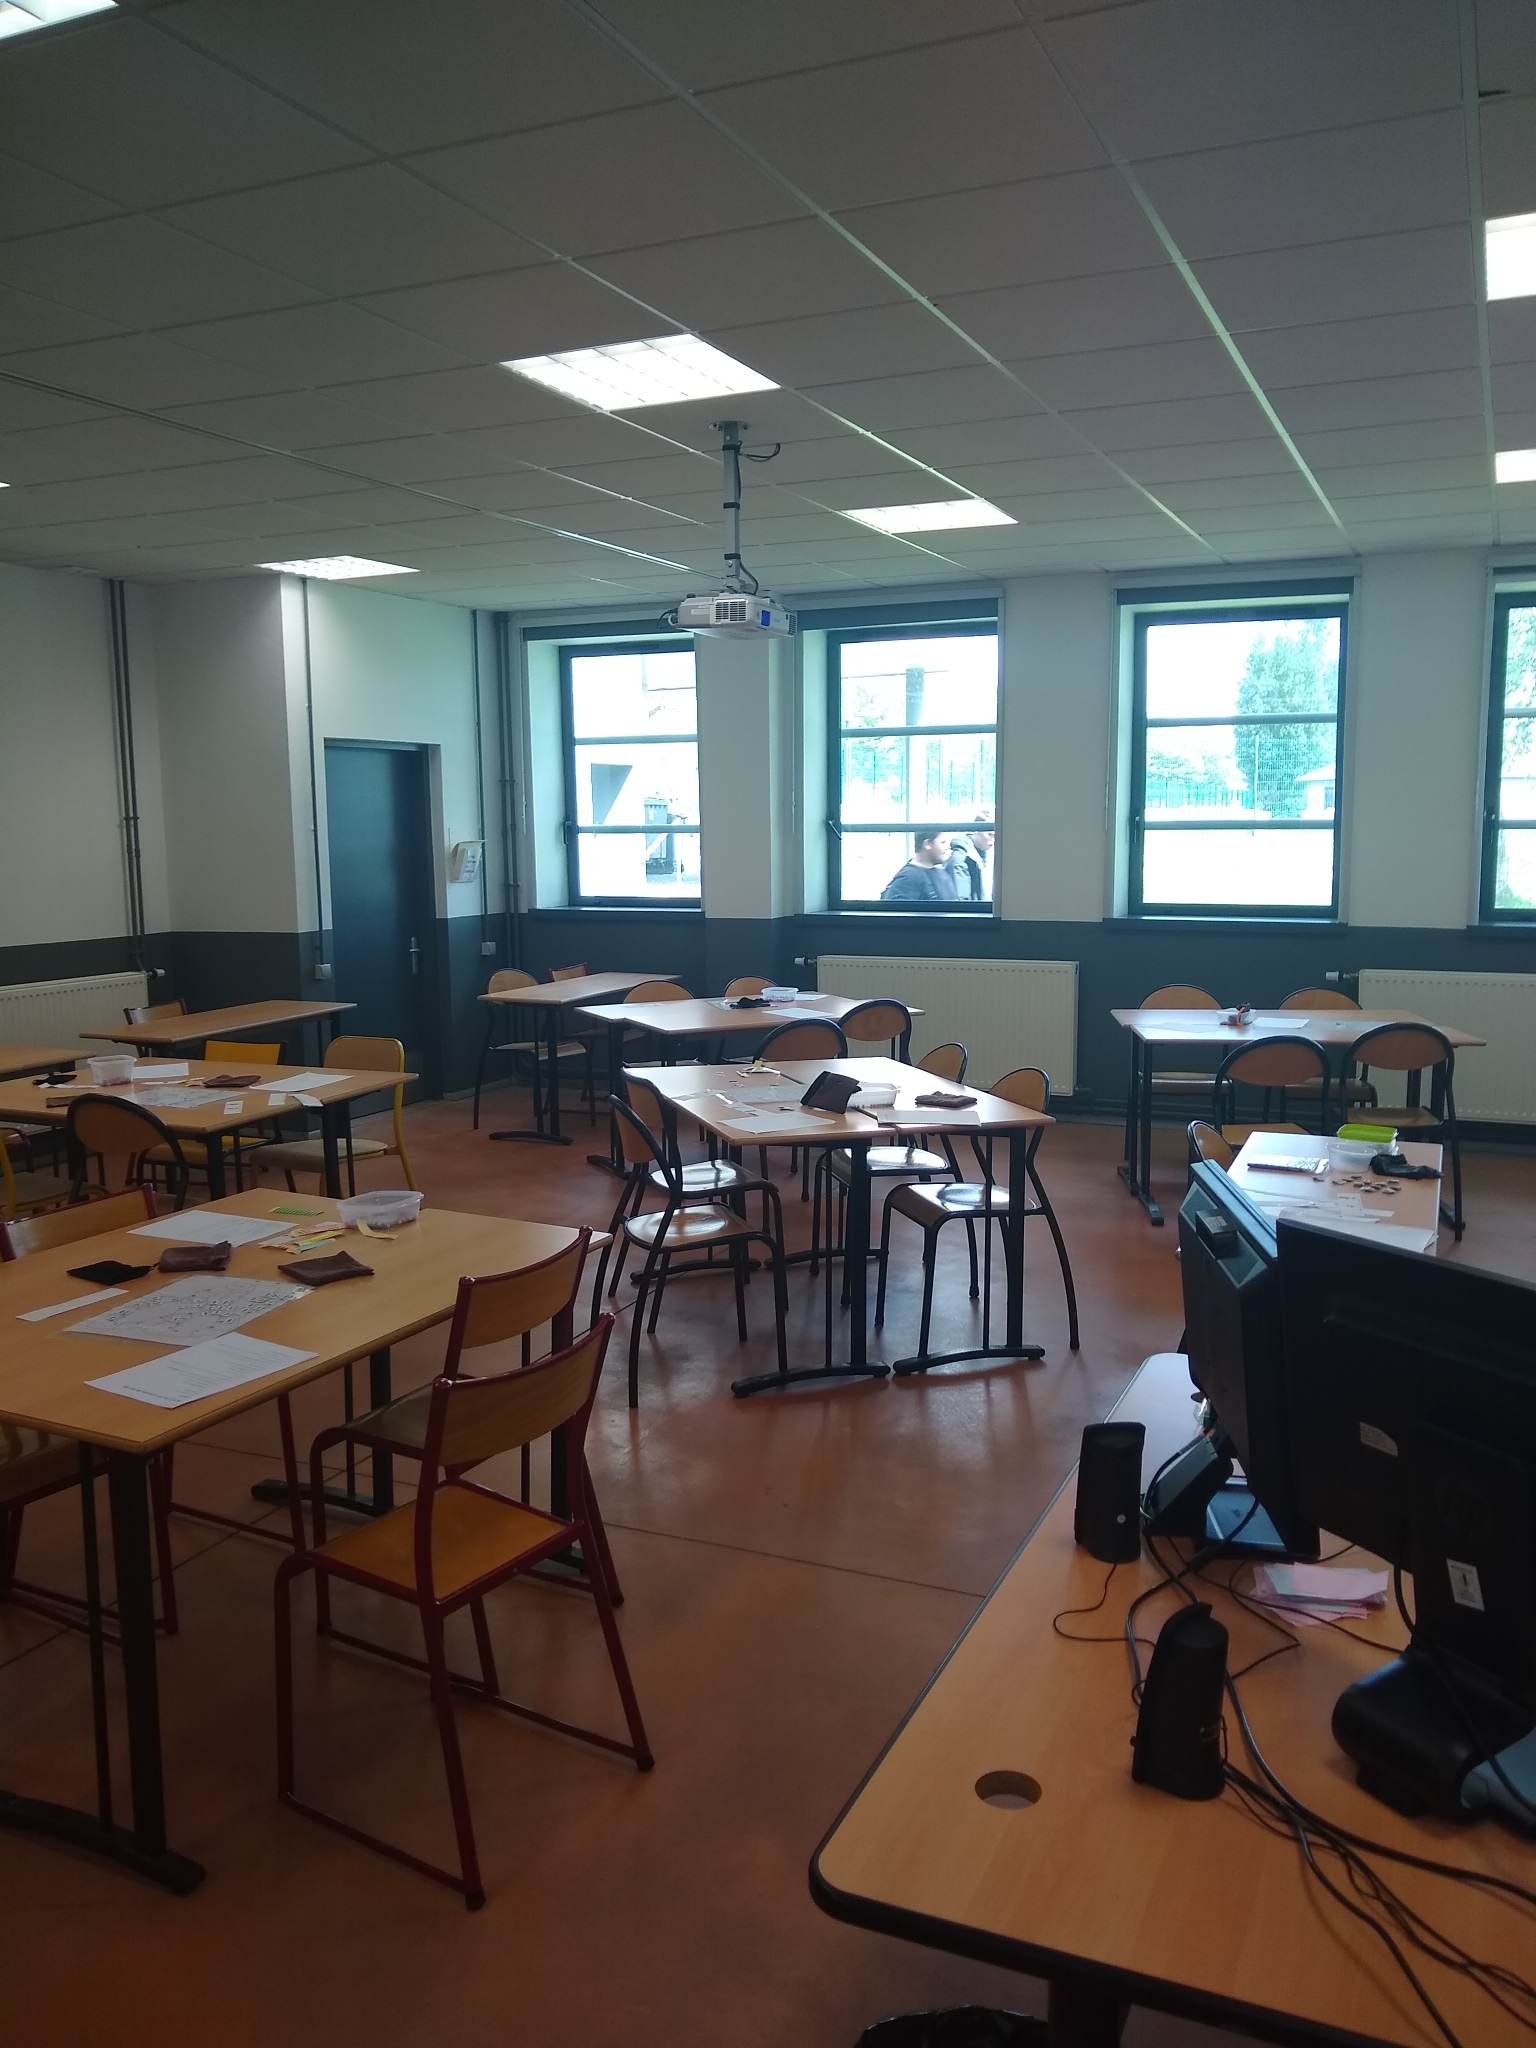
\includegraphics{./img/strategie/autre/ilots.jpg}
\caption{Photo de classe formée en îlots}
\end{figure}

\hypertarget{outils-de-gestion-de-classe}{%
\paragraph{Outils de gestion de
classe}\label{outils-de-gestion-de-classe}}

La répartition des groupes, la gestion du temps et du bruit se fait à
l'aide de l'application web \href{https://ladigitale.dev/digiscreen/}{La
Digitale}.

\hypertarget{collecte-des-donnuxe9es}{%
\subsection{Collecte des données}\label{collecte-des-donnuxe9es}}

L'analyse des données recueillies doit permettre de valider des
hypothèses. Comme celle d'afficher une différence sur la compréhension
des mécanismes de l'intelligence artificielle entre le début et la fin
de la séquence, l'objectif étant de répondre à la problèmatique.

Les données exploitées sont récupérées via un questionnaire dans un
premier temps puis via une évaluation de compétences dans un deuxième
temps.

\hypertarget{via-un-questionnaire}{%
\subsubsection{Via un questionnaire}\label{via-un-questionnaire}}

Les données à analyser sont les réponses d'un questionnaire distribué en
début et fin de séance. Il y aura donc un même questionnaire soumis deux
fois aux élèves.

Le questionnaire est proposé en \hyperref[sec:annexe5]{annexe 5}.

Le questionnaire est sous forme de QCM et propose 14 questions d'ordre
de culture générale sur l'intelligence artificielle et quelques
questions plus spécifiques aux algorithmes d'apprentissage par
renforcement.

L'objectif serait de déterminer une différence croissante entre les
résultats de la première évaluation et les résultats de la seconde pour
prouver un potentiel impact de l'activité sur l'apprentissage des
élèves.

On note \(Notes_1\) et \(Notes_2\) l'ensemble des notes receuillies
respectivement la première fois et la seconde fois. Les échantillons
sont indépendants, la moyenne devrait donc suivre une loi normale.

Les résultats sont à caractère quantitatifs, ce sont des notes sur 14.
Il s'agit de résultats d'une même classe donc ils sont appariés.

\hypertarget{test-de-student}{%
\paragraph{Test de Student}\label{test-de-student}}

Afin de démontrer une quelconque différence entre les moyennes de
\(Notes_1\) et \(Notes_2\), nous allons utiliser le test de Student.

Le test de Student permet de valider ou rejetter les hypothèses
suivantes :

\begin{itemize}
\item
  Hypothèse nulle \(H_0\) : La moyenne de \(Notes_2\) est inférieure à
  celle de \(Notes_1\).
\item
  Hypothèse alternative \(H_1\) : La moyenne de \(Notes_2\) est
  supérieure à celle de \(Notes_1\).
\end{itemize}

Si \(H_1\) est validée, nous serons en moyen de prouver que la stratégie
a eu un impact sur l'apprentissage des élèves à propos de leur culture
générale sur l'intelligence artificielle.

\hypertarget{test-de-mc-nemar}{%
\paragraph{Test de Mc Nemar}\label{test-de-mc-nemar}}

On souhaite déterminer si l'activité a eu un réel impact précisément sur
l'apprentissage des algorithmes par renforcement.

Pour cela, nous réalisons un premier test de Mc Nemar sur la réponse à
question n°12 (: \emph{``Les algorithmes d'apprentissage par
renforcement sont basés sur une manière naturelle d'apprendre : Oui -
Non''}).

Puis un second test sur la question n°13 (: \emph{``L'idée des
algorithmes d'apprentissage par renforcement est définie sur : La
répétition d'une action jusqu'à ce qu'elle soit satisfaisante. - Le
renforcement d'une action selon une récompense''.})

On effectue les mesures pour les deux tests :

\begin{itemize}
\item
  Avant l'activité, \(n_1\) élèves ont répondus correctement à la
  question n°12, \(p_1\) élèves n'ont pas répondus correctement.
\item
  Après l'activité, \(n_2\) élèves ont répondu correctement à la
  question n°13, \(p_2\) élèves n'ont pas répondus correctement.
\end{itemize}

Si \(n_2 > n_1\) pour les deux tests, nous serons en moyen de prouver
que l'activité a eu un impact sur l'apprentissage des élèves à propos
des algorithmes d'apprentissage par renforcement.

\hypertarget{tableau-de-contingence-sur-la-question-n5}{%
\paragraph{Tableau de contingence sur la question
n°5}\label{tableau-de-contingence-sur-la-question-n5}}

Nous souhaitons savoir pour les élèves qui ont déjà entendu les termes
``machine learning'' ont une meilleure note que les élèves qui ne l'ont
jamais entendu.

Ce type d'hypothèse permettrait de savoir s'il y a une corrélation entre
la réponse à cette question et la note de l'élève.

\begin{itemize}
\item
  Hypothèse nulle \(H_0\) : Il y a une corrélation entre la question n°5
  et la note de l'élève.
\item
  Hypothèse alternative \(H_1\) : Il n'y a pas de corrélation entre la
  question n°5 et la note de l'élève.
\end{itemize}

Pour cela, nous utilisons un tableau de contingence :

\begin{tabular}{|c|c|c|}
\hline
Tableau de contingence&Notes < 10&Notes >= 10\\
\hline
Nombre de réponses correctes& & \\
\hline
Nombre de réponses incorrectes& & \\
\hline
\end{tabular}

Ce test pourrait affirmer que les élèves qui ont déjà entendu ces termes
n'ont pas nécessairement une meilleure note.

\hypertarget{tableau-de-contingence-sur-la-question-n14}{%
\paragraph{Tableau de contingence sur la question
n°14}\label{tableau-de-contingence-sur-la-question-n14}}

Nous souhaitons savoir s'il y a une corrélation entre la réponse à la
dernière question ( : \emph{Avez-vous peur de l'intelligence
artificielle ? Oui - Non}) et la note de l'élève.

\begin{itemize}
\item
  Hypothèse nulle \(H_0\) : Il n'y a pas de corrélation entre la
  question n°14 et la note de l'élève.
\item
  Hypothèse alternative \(H_1\) : Il y a une corrélation entre la
  question n°14 et la note de l'élève.
\end{itemize}

Pour cela, nous utilisons un tableau de contingence :

\begin{tabular}{|c|c|c|}
\hline
Tableau de contingence&Notes < 10&Notes >= 10\\
\hline
Nombre de réponses correctes& & \\
\hline
Nombre de réponses incorrectes& & \\
\hline
\end{tabular}

Ce test permettrait d'affirmer que les élèves qui, globalement ont une
moins bonne note, ont plus facilement peur de l'intelligence
artificielle.

Et ainsi, permettrait de vérifier la célèbre citation de Guy de
Maupassant : ``On a peur que de ce qu'on ne comprend pas''.

\hypertarget{via-les-compuxe9tences}{%
\subsubsection{Via les compétences}\label{via-les-compuxe9tences}}

On peut également savoir si l'activité a eu un impact sur les
savoirs-faire des élèves notamment en les observant pendant et en
évaluant leurs compétences.

L'évaluation est individuelle pour chaque élèves et sont regroupées dans
un tableau de compétences des savoirs-faire :

\begin{tabular}{|c|c|c|}  
\hline   
Axes&Critères&Descriptifs\\
\hline   
\multirow{5}{*}{Algorithme}&
Réinvestissement des
&L'élève connaît les fonctionnements \\
&connaissances de base
& des constructions élémentaires\\

\cline{2-3}

&Réinvestissement des
&L'élève fait le lien entre ses connaissances sur\\
&connaissances sur les
&les algorithmes d'apprentissage par renforcement \\
&algorithmes d'apprentissage
&et l'algorithme des colonies de fourmis\\

\hline

Analyse&Problème du chemin
&L'élève analyse le problème du\\
&de poids minimum
&chemin de poids minimum dans un graphe\\

\hline
\multirow{3}{*}{Activité}
&Appropriation de la
&L'élève s'approprie le plateau et \\
&situation
&ses différents supports,\\
& &l'élève effectue l'algorithme des\\
& &colonies de fourmis sur ce plateau\\

\cline{2-3}

&Analyse d'une solution
&L'élève voit apparaître sur son plateau\\
& &une solution et sait l'analyser\\

\cline{2-3}

&Communication
&L'élève sait décrire les résultats qu'il a obtenu\\

\hline
\end{tabular}

Cette activité en groupe est également l'occasion d'évaluer les élèves
sur leurs compétences à savoir travailler en groupe :

\begin{tabular}{|c|c|c|}  
\hline   
Axes&Critères&Descriptifs\\
\hline   
\multirow{2}{*}{Communication}
&Communication claire
&L'élève communique de manière concise, claire\\
& &et efficace\\
\cline{2-3}
&Partage&L'élève fait part de ses réflexions,\\
& &de ses idées\\

\cline{2-3}

&Langage approprié
&L'élève utilise un langage adapté à la\\
&&situation\\

\cline{2-3}

&Respect
&L'élève écoute activement, respecte les\\
& &temps de paroles\\
\hline
Altruisme&Solidarité&L'élève favorise l'entraide\\
\hline

\multirow{2}{*}{Responsabilité}&Dans son travail
&L'élève accomplit sa part de travail\\

\cline{2-3}

&Dans son groupe
&L'élève est plutôt un élément moteur\\
&&qu'un élément perturbateur\\
\hline

\multirow{2}{*}{Collaboration}
&Répartition des tâches
&Les tâches sont divisées de\\
&&manière équitable\\

\cline{2-3}

&Mutualisation&Les élèves mutualisent de manière efficace\\
\hline
\end{tabular}

\hypertarget{ruxe9sultats-et-analyse}{%
\section{Résultats et analyse}\label{ruxe9sultats-et-analyse}}

\hypertarget{conclusion}{%
\section{Conclusion}\label{conclusion}}

mes conclusions

\hypertarget{annexes}{%
\section{Annexes}\label{annexes}}

\hypertarget{annexe-1}{%
\subsection{Annexe 1}\label{annexe-1}}

Programme python, dilemme de l'exploration - exploitation selon une
probabilité epsilon

\begin{lstlisting}[language=Python, numbers=left, label=dilemme_exploration_exploitation]
import random
import matplotlib.pyplot as plt

def initialise_filons(n : int)->list:
    """
    :param n (int): Nombre d elements
    :return list: Renvoie une liste de nombres aleatoires de taille n
    """
    return [random.randint(1,20) for _ in range(n)]

def explore(filons_reels : list)->int:
    """
    :param filons_reels (list): Liste des filons existant
    :return int: Renvoie un indice aleatoire de la liste filons_reels
    """
    return random.randint(0, len(filons_reels)-1)

def exploite(filons_connus : list)->int:
    """
    :param filons_connus (list): Liste des filons que l'on connait
    :return int: Renvoie l'indice du maximum de la liste filons_connus
    """
    ind_max = 0
    for i in range(len(filons_connus)):
        if filons_connus[i] > filons_connus[ind_max] :
            ind_max = i
    return ind_max

def dilemme_exploration_exploitation(n : int,epsilon : float)->float:
    """
    :param n (int): Nombre de filons
    :param epsilon (float): probabilite epsilon
    :return float: Renvoie la moyenne des recompenses selon une probabilite epsilon d'explorer ou d'exploiter
    """
    filons_reels = initialise_filons(n)
    filons_connus = [0 for _ in range(n)]
    recompense_ieme = 0
    list_recompenses = []
    moyenne = []
    for _ in range(500):
        if random.uniform(0,1) <= epsilon :
            ind = explore(filons_reels)
            filons_connus[ind] = filons_reels[ind]
        else :
            ind = exploite(filons_connus)
        recompense_ieme = filons_connus[ind]
        list_recompenses.append(recompense_ieme)
        moyenne.append(sum(list_recompenses)/len(list_recompenses))
    return moyenne

def stats():
    """
    Creation d'un graphique representant la moyenne des recompenses pour 3 probabilites epsilon
    """
    n = 20
    eps_001 = dilemme_exploration_exploitation(n, 0.01)
    eps_01 = dilemme_exploration_exploitation(n, 0.1)
    eps_03 = dilemme_exploration_exploitation(n, 0.3)

    plt.plot(eps_001, label="0.01")
    plt.plot(eps_01 , label="0.1")
    plt.plot(eps_03 , label="0.3")

    plt.title("Moyenne des recompenses en fonction d'epsilon")
    plt.legend()
    plt.ylabel("Moyenne des recompenses")
    plt.xlabel("Nombres d'iterations")
    #plt.savefig("../img/moy_exploration_exploitation.png")
    plt.show()
\end{lstlisting}

\hypertarget{annexe-2}{%
\subsection{Annexe 2}\label{annexe-2}}

Programme Python, dilemme de l'exploration - exploitation, selon une
probabilité epsilon et utilisant la méthode d'estimation d'actions

\begin{lstlisting}[language=Python, numbers=left, label=exploration_exploitation_estimations]
import random
import matplotlib.pyplot as plt

def initialise_filons(n : int)->list:
    """
    :param n (int): Nombre d'elements
    :return list: Renvoie une liste de nombres aleatoires de taille n
    """
    return [random.randint(1,100) for _ in range(n)]

def initialise_estimations(filons : list)->list:
    """
    :param filons (list): Une liste representant les filons reels
    :return list: Renvoie une liste d'estimations aleatoires des filons reels
    """
    return [random.randint(1,100) for i in range(len(filons))]

def converge(estimations : list, filons : list, i : int)->float:
    """
    :param estimations (list): Liste representant les estimations des filons
    :param filons (list): Liste representant les filons reels
    :param i (int): Un indice i
    :return float: Renvoie une nouvelle valeur d'estimations a l'indice i qui converge vers la valeur reelle du filon 
    """
    v = filons[i] - estimations[i]
    return estimations[i] + (v/2)

def explore(filons : list)->int:
    """
    :param filons (list): Liste representant les filons reels
    :return int: Renvoie un indice aleatoire
    """
    return random.randint(0, len(filons)-1)

def exploite(estimations : list)->int:
    """
    :param estimations (list): Liste representant les estimations
    :return int: Renvoie l'indice de la plus haute estimation
    """
    ind_max = 0
    for i in range(len(estimations)):
        if estimations[i] > estimations[ind_max] :
            ind_max = i
    return ind_max

def exploration_exploitation_estimations(filons : list, estimations : list, epsilon : float)->float:
    """
    :param filons (list): Liste representant les filons reels
    :param estimations (list): Liste representant les estimations
    :param epsilon (float): Probabilite espilon
    :return float: Renvoie une moyenne des recompenses selon la methode d'estimation d'actions
    """
    recompense_ieme = 0
    list_recompenses = []
    moyenne = []
    for _ in range(1000):
        if random.uniform(0,1) <= epsilon :
            ind = explore(filons)
            estimations[ind] = converge(estimations, filons, ind)
        else :
            ind = exploite(estimations)
        recompense_ieme = filons[ind]
        list_recompenses.append(recompense_ieme)
        moyenne.append(sum(list_recompenses)/len(list_recompenses))
    return moyenne

def stats():
    """
    Creation d'un graphique representant les courbes des moyennes des recompenses
    """
    n = 10
    filons = initialise_filons(n)
    estimations = initialise_estimations(filons)
    eps_0 = exploration_exploitation_estimations(filons, estimations, 0)
    eps_01 = exploration_exploitation_estimations(filons, estimations, 0.1)

    plt.plot(eps_0, label="0")
    plt.plot(eps_01 , label="0.1")

    plt.title("Moyenne des recompenses en fonction d'epsilon")
    plt.legend()
    plt.ylabel("Moyenne de la recompense")
    plt.xlabel("Nombres d'iterations")
    #plt.savefig("../img/moy_methode_estimation_action.png")
    plt.show()
\end{lstlisting}

\hypertarget{annexe-3}{%
\subsection{Annexe 3}\label{annexe-3}}

Programme Python modelisant l'algorithme des Colonies de fourmis

\begin{lstlisting}[language=Python, numbers=left, label=colonies_fourmis]
# author : Boddaert Theo
# title: L'apprentissage par renforcement
# date: Annee scolaire 22/23

import random
import matplotlib.pyplot as plt

l_aretes = [('Colonie','B',2),('Colonie','C',3),('Colonie','D',4),
            ('B','E',3),('B','F',3),
            ('C','A',4),('D','A',5),
            ('A','Nourriture',5),('E','Nourriture',2),('F','Nourriture',8)]
nb_fourmis_activite = 50
nb_fourmis_demo = 500
t_evaporation = 8
chemin_gagnant = ['Colonie','B','E','Nourriture']


#------Classe Graphe---------

class Graph:
    def __init__(self):
        """
        Constructeur : Initialise un graphe vide sous forme de liste d'adjacence
        """
        self.adj = {}

    def ajoute_sommet(self,s : str):
        """
        :param s (str): un sommet
        Ajoute au graphe le sommet s
        """
        self.adj[s] = []

    def ajoute_arete(self,arete : list,pheromones=1):
        """
        :param arete (list): une liste representant une arete, elle comprend une source, une arrivee et un nombre de case
        :param pheromones (int): une pheromone initialisee a 1
        Ajoute au graphe une arete
        """
        source = arete[0]
        arrivee = arete[1]
        nb_cases = arete[2]
        if source not in self.adj :
            self.ajoute_sommet(source)
        if arrivee not in self.adj :
            self.ajoute_sommet(arrivee)
        self.adj[source].append({"arrivee" : arrivee, "nombre de case" : nb_cases, "pheromones" : pheromones})
        self.adj[arrivee].append({"arrivee" : source, "nombre de case" : nb_cases, "pheromones" : pheromones})

    def voisins(self,s : str)->list:
        """
        :param s (str): un sommet
        :return list: la liste des voisins de s
        """
        return self.adj[s]

    def get_indice_voisin(self,source : str, arrivee : str)->int:
        """
        :param source (str): le sommet source
        :param arrivee (str): le sommet d'arrivee
        :return int: l'indice du sommet d'arrivee dans la liste des voisins du sommet source
        """
        for i in range (len(self.voisins(source))):
            if self.adj[source][i]["arrivee"] == arrivee :
                return i

    def __str__(self):
        """
        :return str: Affiche le graphe
        """
        res = ""
        for k,val in self.adj.items():
            res = res + str(k) +" : \n"
            for a in val:
                res = res + "   " + str(a)+"\n"
        return res

#------Classe Fourmi----------

class Fourmi:
    def __init__(self,numero : int,s_de_depart : str):
        """
        Constructeur : Initialise une fourmi a partir d'un numero de fourmi et d'un sommet de depart
        """
        self.numero = numero
        self.chemin = [s_de_depart]
        self.nb_cases = 0
        self.nb_cases_retour = 0
        self.retour = False

    def avancer(self):
        """
        Avance d'une case la fourmi
        """
        self.nb_cases -= 1

    def revenir(self):
        """
        Avance d'une case la fourmi lorsqu'elle revient a la colonie
        """
        self.nb_cases_retour -= 1

    def est_sur_sommet(self)->bool:
        """
        :return booleen: Renvoie True si la fourmi est sur un sommet, False sinon
        """
        return self.nb_cases == 0

    def est_sur_nourriture(self)->bool:
        """
        :return booleen: Renvoie True si la fourmi est sur le sommet de nourriture, False sinon
        """
        return self.chemin[-1] == 'Nourriture'

    def est_revenue(self):
        """
        :return booleen: Renvoie True si la fourmi est revenue a la colonie, False sinon
        """
        return self.nb_cases_retour == 0

    def __str__(self):
        """
        :return str: Affiche la fourmi
        """
        return str(self.numero) + " : "+ str(self.chemin)+ str(self.nb_cases)

#-------Initialisation du model ----------

def initialise_model(l_aretes : list)->dict:
    """
    :param l_aretes (list): Liste d'aretes
    :return dict: Construit un graphe selon l_aretes
    """
    model = Graph()
    for a in l_aretes :
        model.ajoute_arete(a)
    return model

def affiche_model(l_aretes : list):
    """
    :param l_aretes (list): Liste d'aretes
    Affiche ou enregistre une representation du graphe
    """
    g = nx.Graph()
    g.add_weighted_edges_from(l_aretes)
    pos = nx.planar_layout(g)
    nx.draw(g, with_labels=True, node_color='skyblue', edge_cmap=plt.cm.Blues, pos = pos)
    edge_labels = dict([((u,v,),d['weight'])
        for u,v,d in g.edges(data=True)])
    nx.draw_networkx_edge_labels(g,pos,edge_labels=edge_labels,label_pos = 0.5, font_color='red', rotate = True)
    #plt.savefig("../img/visualisation_graph.png")
    plt.show()

#-----Colonies de fourmis---------

def choix_voisin(model : dict,sommet_courant : str)->str:
    """
    :param model (dict): Graphe G represente par une liste d'adjacence
    :param sommet_courant (str): Un sommet u de G
    :return str: un sommet aleatoire voisin de u
    """
    voisins = model.voisins(sommet_courant)
    voisins_nom = [v["arrivee"] for v in voisins]
    voisins_pheromones = [v["pheromones"] for v in voisins]
    return random.choices(voisins_nom, weights=voisins_pheromones, k=len(voisins_pheromones))[0]

def renforcer_chemin(model : dict,chemin : list):
    """
    :param model (dict): Graphe G represente par une liste d'adjacence
    :param chemin (list): Liste contenant tous les sommets que la fourmi a traverse
    """
    for i in range(0,len(chemin)-1):
        iv = model.get_indice_voisin(chemin[i],chemin[i+1])
        model.adj[chemin[i]][iv]["pheromones"] += 1

def calcul_retour(model : dict,chemin : list)->int:
    """
    :param model (dict): Graphe G represente par une liste d'adjacence
    :param chemin (list): Liste contenant tous les sommets que la fourmi a traverse
    :return int: La somme du nombre des cases du chemin
    """
    nb_cases_retour = 0
    for i in range(len(chemin)-1):
        nb_cases_retour += model.adj[chemin[i]][model.get_indice_voisin(chemin[i],chemin[i+1])]["nombre de case"]
    return nb_cases_retour

def evaporation(model : dict):
    """
    :param model (dict): Graphe G represente par une liste d'adjacence
    Enleve une pheromone sur chaques sommets du graphe G
    """
    for k in model.adj :
        for i in range(len(model.adj[k])):
            if model.adj[k][i]["pheromones"] > 1:
                model.adj[k][i]["pheromones"] -= 1

def colonie_de_fourmis(model : dict, t_evaporation : int, nb_fourmis : int)->list:
    """
    :param model (dict): Graphe G represente par une liste d'adjacence
    :param t_evaporation (int): Frequence d'evaporation initialise a 8
    :param nb_fourmis (int): Le nombre de fourmis deployees
    :return list: Effectue l'algorithme des colonies de fourmis et renvoie la liste des chemins empruntes par les fourmis
    """
    chemins_pour_chaques_fourmis = []
    fourmilliere = 'Colonie'
    nourriture = 'Nourriture'
    liste_fourmis = []
    for i in range(nb_fourmis):
        liste_fourmis.append(Fourmi(i,fourmilliere))
        for f in liste_fourmis :
            if f.retour :
                f.revenir()
                if f.est_revenue():
                    renforcer_chemin(model,f.chemin)
                    chemins_pour_chaques_fourmis.append(f.chemin)
                    liste_fourmis.remove(f)
            if f.est_sur_sommet():
                if f.est_sur_nourriture() and not f.retour :
                    f.retour = True
                    f.nb_cases_retour = calcul_retour(model,f.chemin)
                else :
                    sommet_suivant = choix_voisin(model,f.chemin[-1])
                    ind_sommet_suivant = model.get_indice_voisin(f.chemin[-1],sommet_suivant)
                    f.nb_cases = model.adj[f.chemin[-1]][ind_sommet_suivant]["nombre de case"]
                    if sommet_suivant in f.chemin :
                        ind = f.chemin.index(sommet_suivant)
                        f.chemin = f.chemin[:ind]
                    f.chemin.append(sommet_suivant)  
            f.avancer()          
        if i%t_evaporation == 0:
            evaporation(model)
    return chemins_pour_chaques_fourmis

#------Optimisation des parametres---------

def reussite_par_parties_fourmis():
    """
    Creation d'un graphique representant le nombre de parties gagnees en fonction du nombre de fourmis
    """
    tab_reussite, tab_echec = [], []
    for test_fourmis in range(50,650,50):
        reussite, echec = 0, 0
        for _ in range(1000):
            chemins_pour_chaques_fourmis = colonie_de_fourmis(initialise_model(l_aretes),t_evaporation, test_fourmis)
            nb_f_md = chemins_pour_chaques_fourmis.count(chemin_gagnant)
            if nb_f_md > len(chemins_pour_chaques_fourmis) - nb_f_md :
                reussite += 1
            else :
                echec += 1
        tab_reussite.append(reussite)
        tab_echec.append(echec)
    barWidth = 0.4
    r1 = range(len(tab_reussite))
    r2 = [x + barWidth for x in r1]
    plt.title("Nombres de parties gagnees et echouees en fonction du nombre de fourmis")
    plt.ylabel("Nombre de parties")
    plt.xlabel("Nombre de fourmis utilisees")
    plt.bar(r1, tab_reussite, width = barWidth, label = "Reussite")
    plt.bar(r2, tab_echec, width = barWidth, label = "Echec")
    plt.xticks([r + barWidth / 2 for r in range(len(tab_reussite))], [nb for nb in range(50,650,50)])
    plt.legend()
    #plt.savefig("../img/optimisation_parametres/nb_parties_fourmis.png")
    plt.show()

def reussite_par_parties_evaporation():
    """
    Graphique representant le nombre de parties gagnees en fonction de la frequence d'evaporation
    """
    tab_reussite, tab_echec = [], []
    for test_evaporation in range(2,15,2):
        reussite, echec = 0, 0
        for _ in range(1000):
            chemins_pour_chaques_fourmis = colonie_de_fourmis(initialise_model(l_aretes),test_evaporation,nb_fourmis_demo)
            nb_f_md = chemins_pour_chaques_fourmis.count(chemin_gagnant)
            if nb_f_md > len(chemins_pour_chaques_fourmis) - nb_f_md :
                reussite += 1
            else :
                echec += 1
        tab_reussite.append(reussite)
        tab_echec.append(echec)
    barWidth = 0.4
    r1 = range(len(tab_reussite))
    r2 = [x + barWidth for x in r1]
    plt.title("Nombres de parties gagnees et echouees en fonction de l'evaporation")
    plt.ylabel("Nombre de parties")
    plt.xlabel("Evaporation tous les x tours")
    plt.bar(r1, tab_reussite, width = barWidth, label = "Reussite")
    plt.bar(r2, tab_echec, width = barWidth, label = "Echec")
    plt.xticks([r + barWidth / 2 for r in range(len(tab_reussite))], [eva for eva in range(2,15,2)])
    plt.legend()
    #plt.savefig("../img/optimisation_parametres/nb_parties_evaporation.png")
    plt.show()

#-------Statistiques--------

def pour_reussite():
    """
    Graphique representant le pourcentage de parties gagnees pour 10 experiences
    """
    tab_pour = []
    for _ in range(10):
        reussite, total = 0, 0
        for _ in range(500):
            chemins_pour_chaques_fourmis = colonie_de_fourmis(initialise_model(l_aretes),t_evaporation,nb_fourmis_demo)
            nb_f_md = chemins_pour_chaques_fourmis.count(chemin_gagnant)
            if nb_f_md > len(chemins_pour_chaques_fourmis) - nb_f_md :
                reussite += 1
            total += 1
        tab_pour.append(int((reussite * 100) / total))
    plt.title("Pourcentage de parties gagnees sur 10 experiences")
    plt.bar(range(len(tab_pour)), tab_pour)
    plt.ylim(top = 100)
    for index,data in enumerate(tab_pour):
        plt.text(x=index , y =data+1 , s=f"{data}% " , fontdict=dict(fontsize=10))
    plt.tight_layout()
    plt.xticks([r for r in range(len(tab_pour))], ["Exp " + str(par) for par in range(0,10)])
    #plt.savefig("../img/statistiques/pourcentage_reussite.png")
    plt.show()

def repartition_fourmis():
    """
    Graphique representant la repartition des fourmis
    """
    nb_f_mc , nb_f_n_mc , nb_f_ni = 0,0,0
    for _ in range(1000) :
        chemins_pour_chaques_fourmis = colonie_de_fourmis(initialise_model(l_aretes),t_evaporation, nb_fourmis_demo)
        nb_f_mc += chemins_pour_chaques_fourmis.count(chemin_gagnant)
        nb_f_n_mc += len(chemins_pour_chaques_fourmis) - chemins_pour_chaques_fourmis.count(chemin_gagnant)
        nb_f_ni += nb_fourmis_demo - len(chemins_pour_chaques_fourmis)
    plt.title("Repartition des fourmis en pourcentage sur 1000 parties")
    plt.pie([nb_f_mc , nb_f_n_mc , nb_f_ni],
            normalize = True,
            autopct = lambda x: str(round(x, 2)) + '%')
    plt.legend(["Fourmis ayant trouve le meilleur chemin", "Fourmis ayant trouve la nourriture mais pas le meilleur chemin" , "Fourmis n'ayant pas trouve la nourriture"])
    #plt.savefig("../img/statistiques/repartition_fourmis.png")
    plt.show()

def moyenne_cumulee():
    """
    Graphique representant la moyenne cumulee du pourcentage de parties gagnee
    """
    pourcentages_reussite = []
    moyennes_reussite = []
    moyenne_cumulee = []
    for _ in range(100):
        for _ in range(100) :
            chemins_pour_chaques_fourmis = colonie_de_fourmis(initialise_model(l_aretes),t_evaporation, nb_fourmis_demo)
            nb_f_md = chemins_pour_chaques_fourmis.count(chemin_gagnant)
            pourcentages_reussite.append(nb_f_md * 100 / len(chemins_pour_chaques_fourmis))

        moyennes_reussite.append(sum(pourcentages_reussite) / len(pourcentages_reussite))
        moyenne_cumulee.append(sum(moyennes_reussite)/len(moyennes_reussite))
        pourcentages_reussite = []
    plt.plot(moyenne_cumulee)
    plt.ylabel("Moyenne des pourcentages de reussite sur 10 parties")
    plt.xlabel("Nombre d'experience")
    plt.title('Moyenne cumulee sur 100 experiences')
    #plt.savefig("../img/statistiques/moy_cumul.png")
    plt.show()

if __name__ == '__main__' :
    #affiche_model(l_aretes)
    model = initialise_model(l_aretes)
    colonie_de_fourmis(model, t_evaporation, nb_fourmis_demo)
    print(model)
\end{lstlisting}

\hypertarget{annexe-4}{%
\subsection{Annexe 4}\label{annexe-4}}

\label{sec:annexe4}Notice de jeu Colonie de Fourmis :

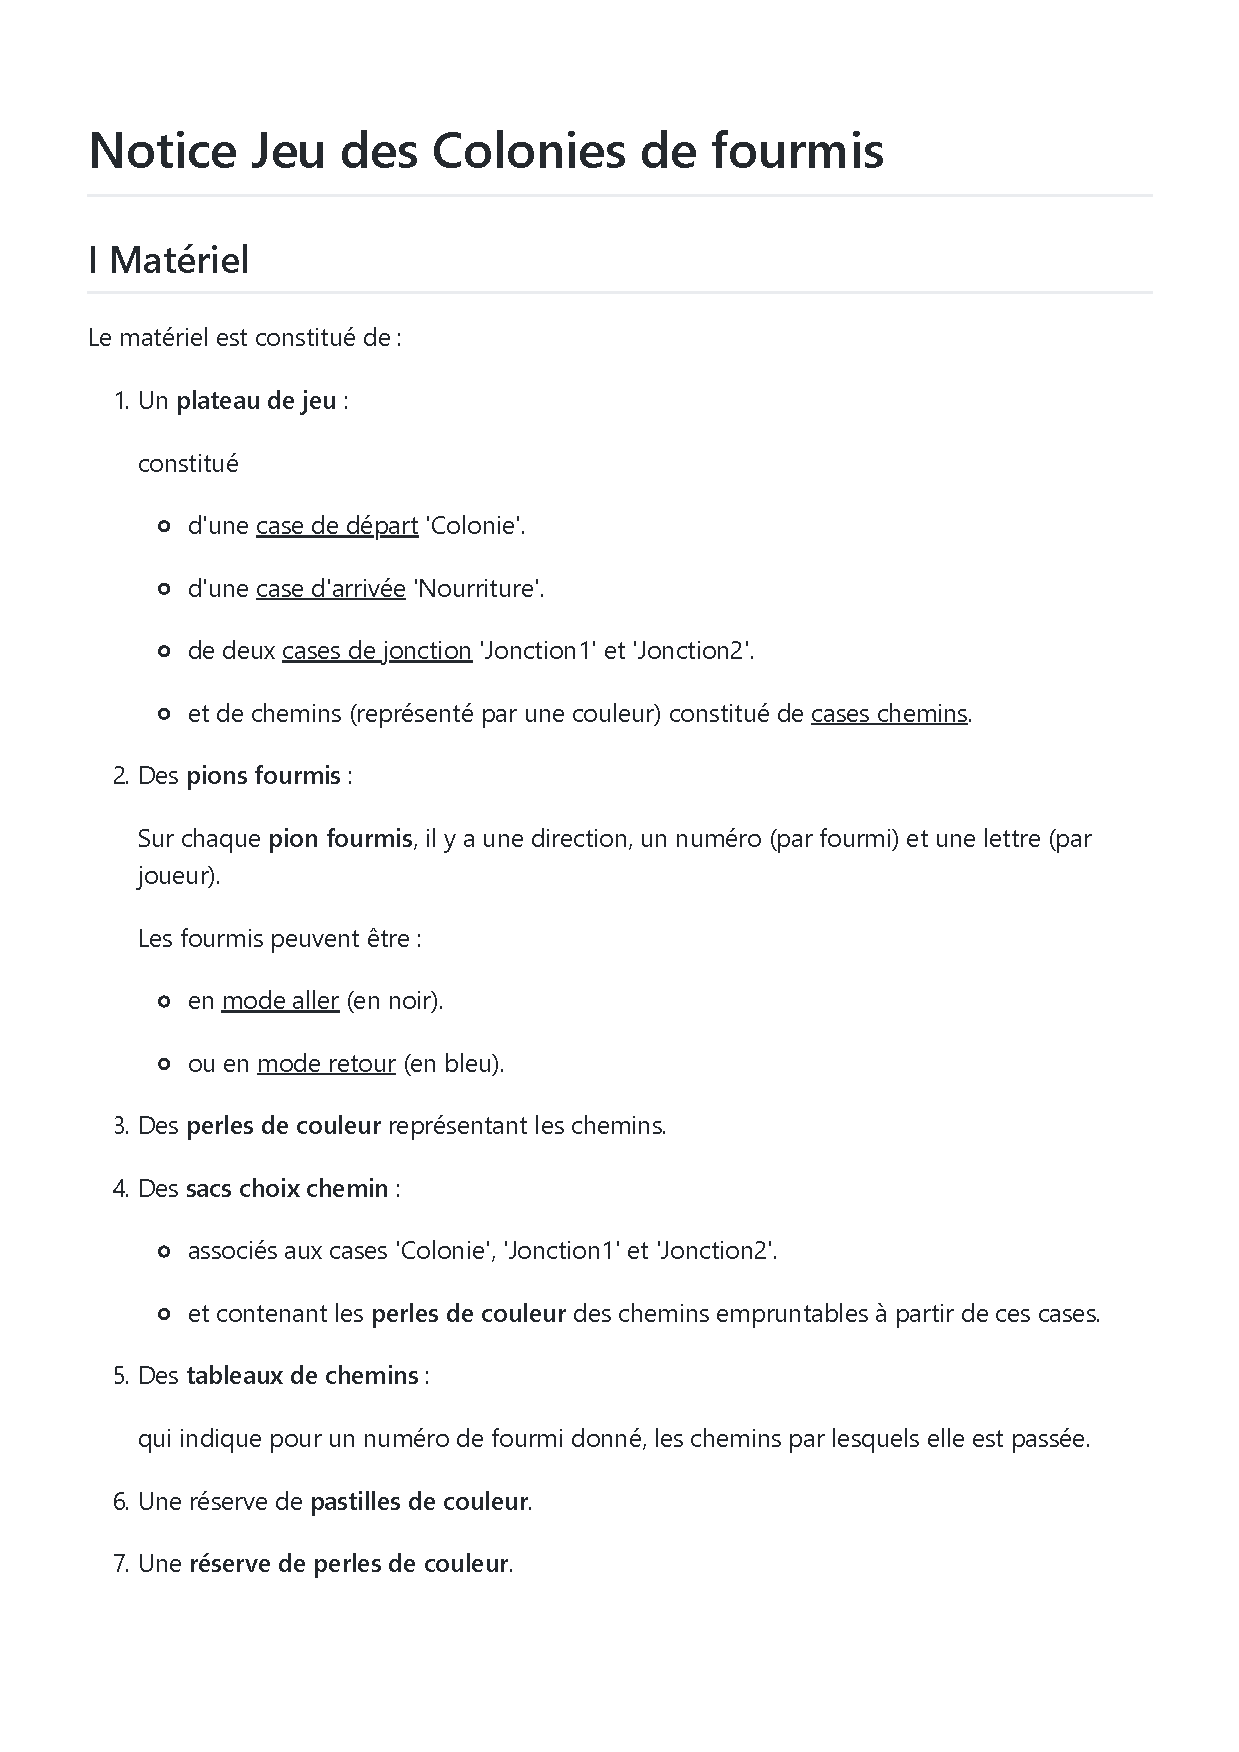
\includepdf[pages=1]{./img/strategie/activite/Notice_Jeu_des_Colonies_de_fourmis.pdf}
\includepdf[pages=2]{./img/strategie/activite/Notice_Jeu_des_Colonies_de_fourmis.pdf}\includepdf[pages=3]{./img/strategie/activite/Notice_Jeu_des_Colonies_de_fourmis.pdf}
\includepdf[pages=4]{./img/strategie/activite/Notice_Jeu_des_Colonies_de_fourmis.pdf}

\hypertarget{annexe-5}{%
\subsection{Annexe 5}\label{annexe-5}}

\label{sec:annexe5}Questionnaire soumis aux élèves :

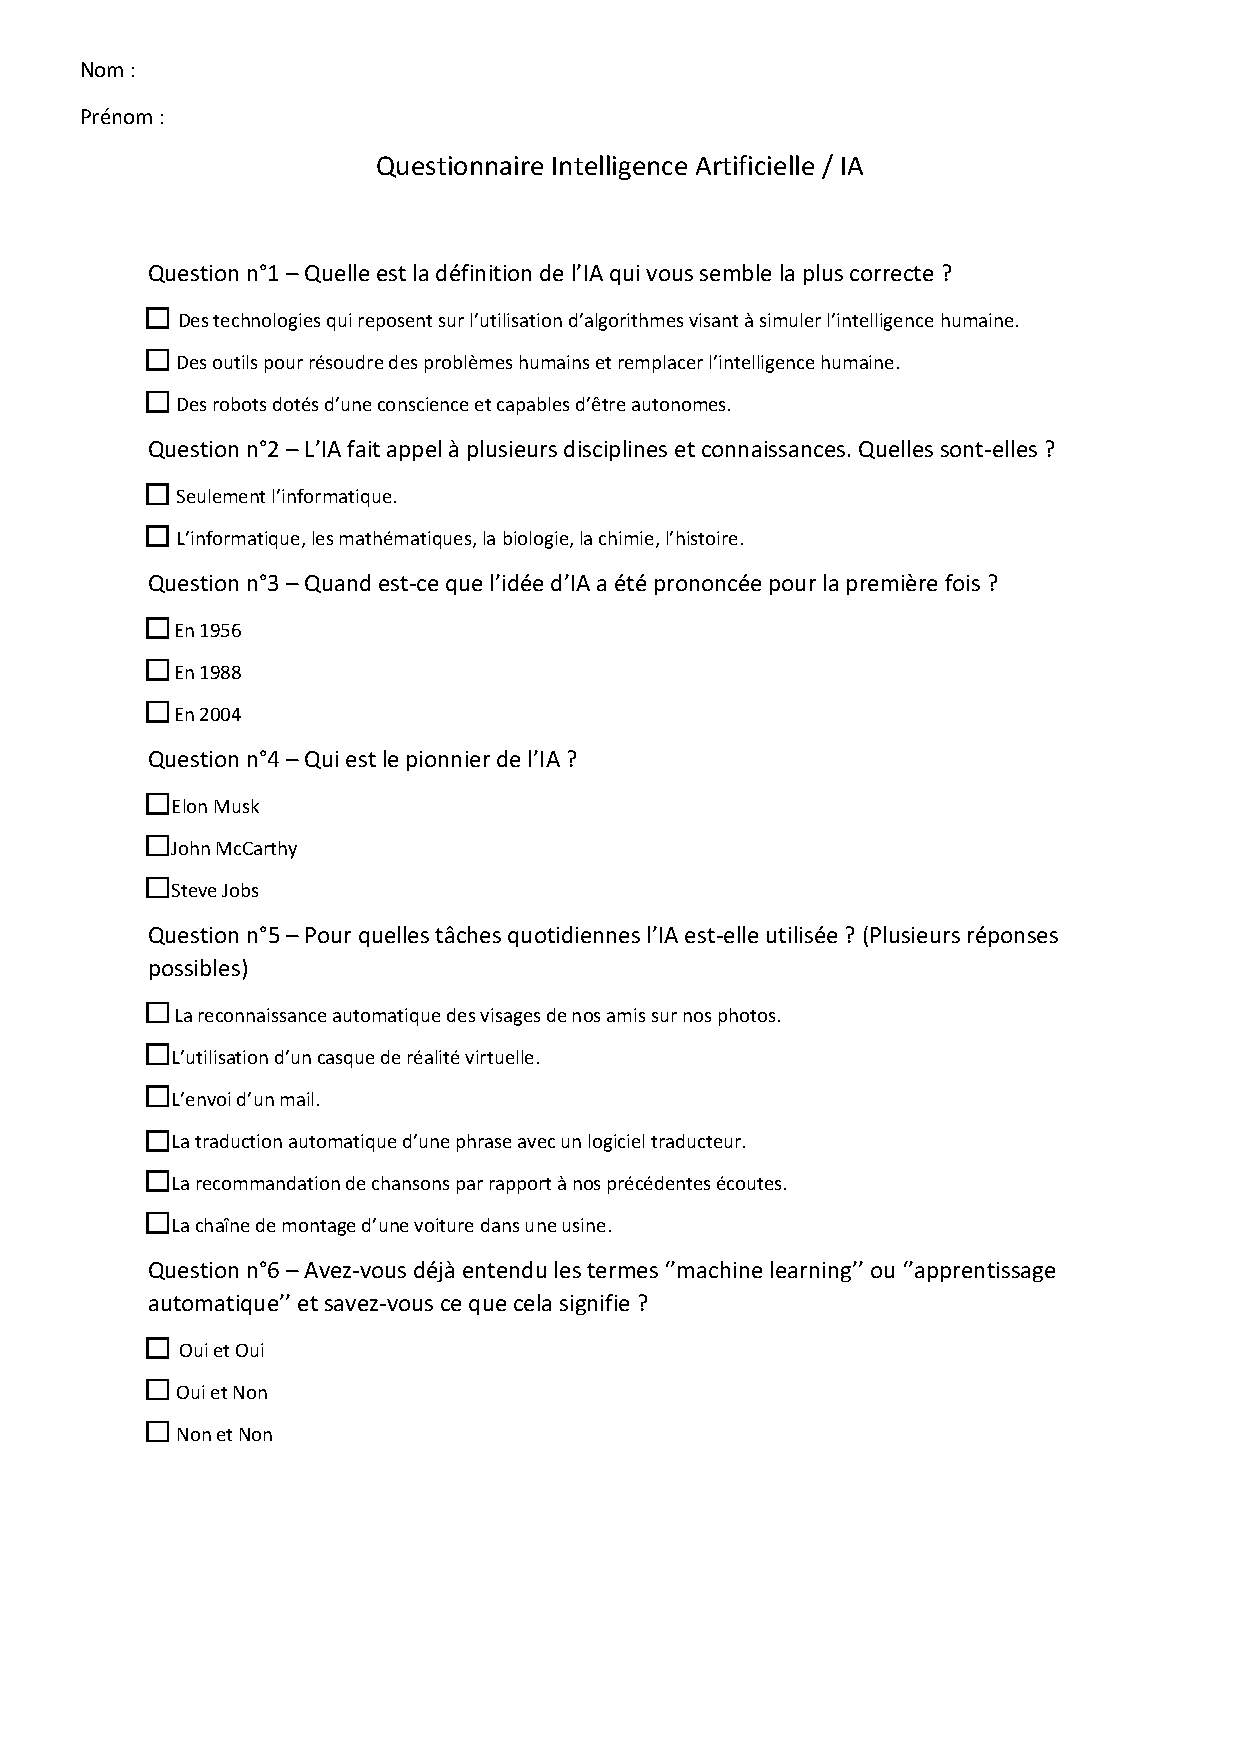
\includepdf[page=1]{./img/strategie/activite/Questionnaire_Intelligence_Artificielle.pdf}
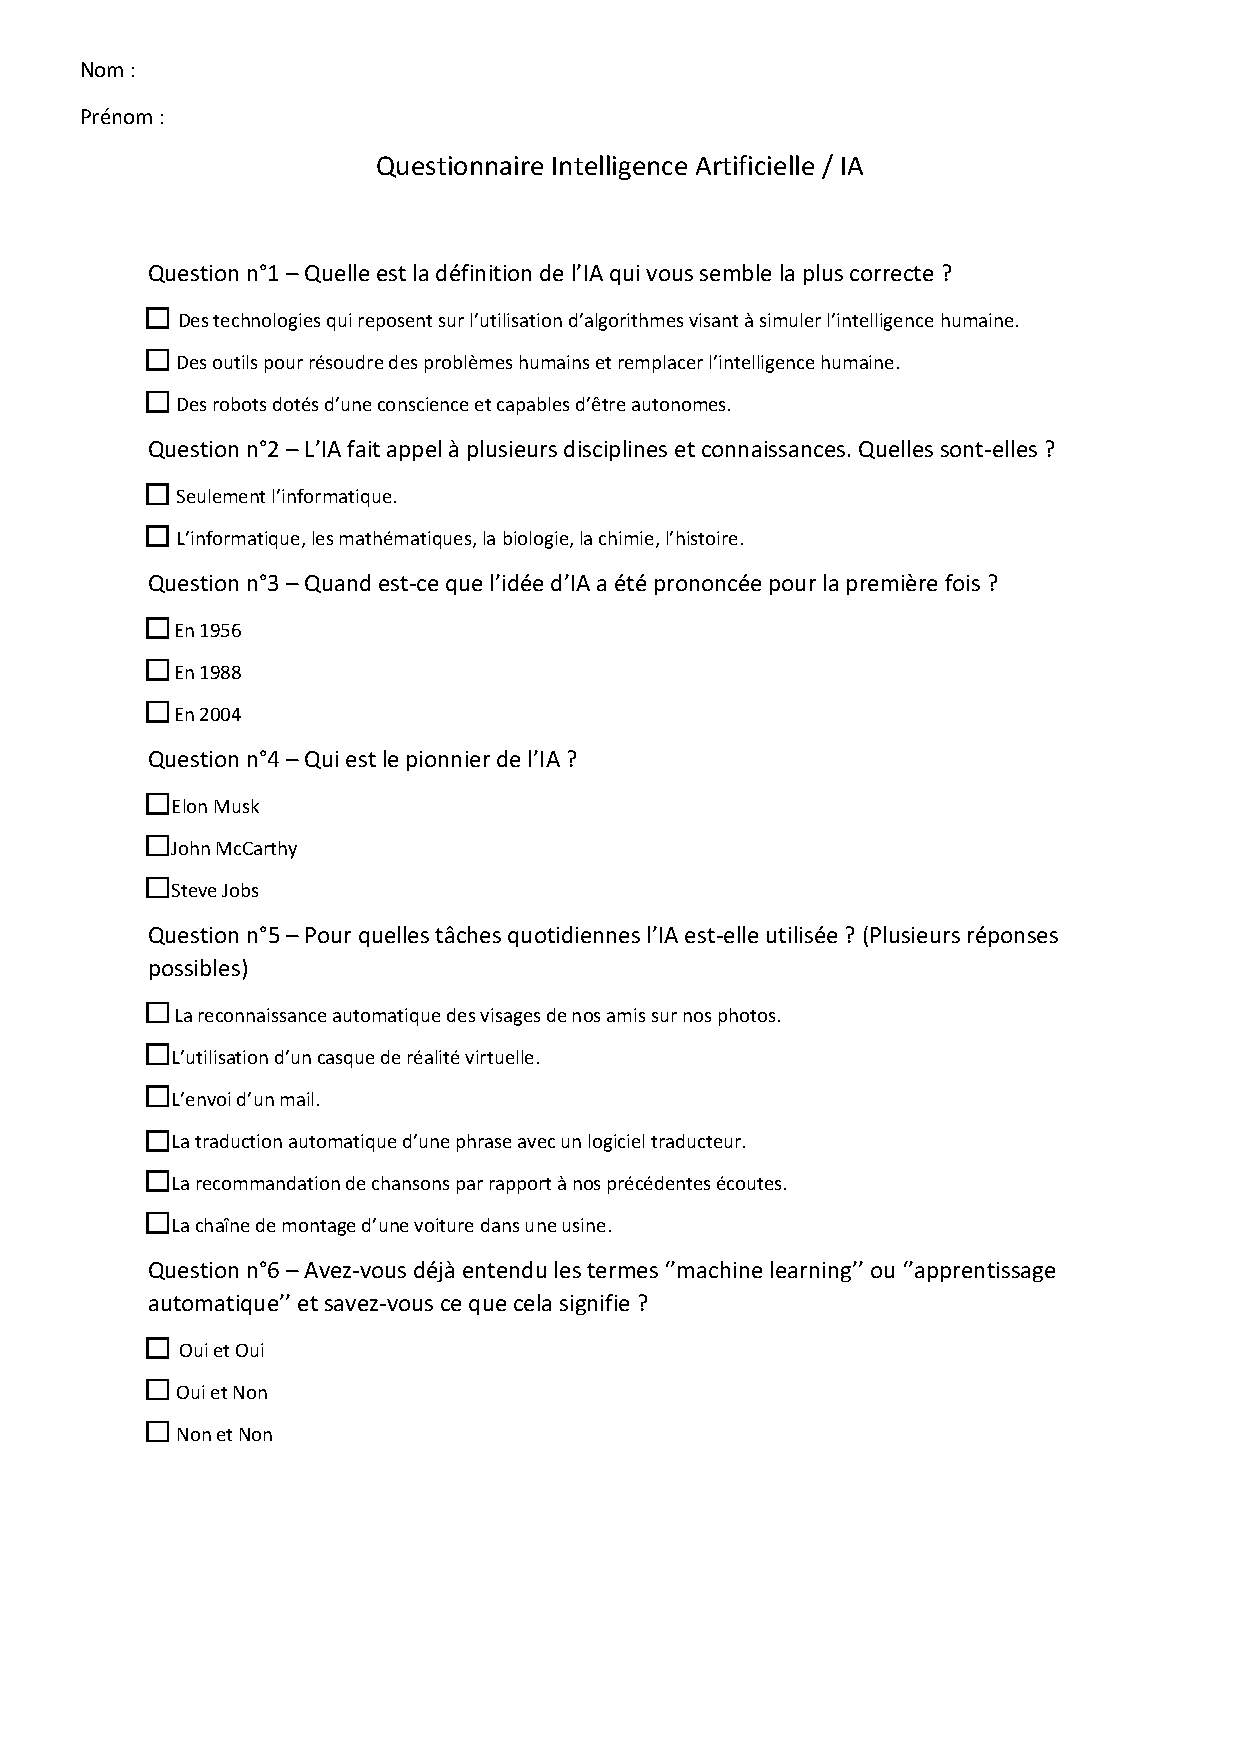
\includepdf[page=2]{./img/strategie/activite/Questionnaire_Intelligence_Artificielle.pdf}

\hypertarget{refs}{}
\begin{CSLReferences}{1}{0}
\leavevmode\vadjust pre{\hypertarget{ref-DistributedOptimizationbyAntColonies}{}}%
A. Colorni, M. Dorigo et V. Maniezzo. 1990. {``Distributed Optimization
by Ant Colonies.''}

\leavevmode\vadjust pre{\hypertarget{ref-DynamicProgrammingandMarkovProcesses}{}}%
Howard, Ronald A. 1960. {``Dynamic Programming and Markov Processes.''}

\leavevmode\vadjust pre{\hypertarget{ref-ExplorationandExploitation}{}}%
March, James G. 1991. {``Exploration and Exploitation in Organization
Learning.''} \emph{Stanford University}.

\leavevmode\vadjust pre{\hypertarget{ref-AlgorithmesDeFourmisArtificiellesApplicationsALaClassificationEtAOptimisation}{}}%
Nonmarché, N. 2000. {``Algorithmes de Fourmis Artificielles :
Applications à La Classification Et à l'optimisation.''}
\emph{Université de Tours}.

\leavevmode\vadjust pre{\hypertarget{ref-NepaliHandwrittenCharacterRecognition}{}}%
Pant, A. Kumar. 2012. {``Off-Line Nepali Handwritten Character
Recognition Using MLP and RBF Neural Networks.''} \emph{Tribhuvan
University}.

\leavevmode\vadjust pre{\hypertarget{ref-ReinforcementLearningAnIntroduction}{}}%
Richard S. Sutton, Andrew G. Barto. 1992. {``Reinforcement Learning : An
Introduction.''} \emph{MIT Press}.

\end{CSLReferences}

\listoftables
\newpage
\listoffigures
\lstlistoflistings

\end{document}
